%%%%%%%%%%%%%%%%%%%% book.tex %%%%%%%%%%%%%%%%%%%%%%%%%%%%%
%
% sample root file for the chapters of your monograph or textbook
%
% Use this file as a template for your own input.
%
%%%%%%%%%%%%%%%% Springer Nature %%%%%%%%%%%%%%%%%%%%%%%%%%

% RECOMMENDED %%%%%%%%%%%%%%%%%%%%%%%%%%%%%%%%%%%%%%%%%%%%%%%%%%%
\documentclass[graybox,envcountchap,sectrefs]{SNmono}

%\usepackage{mathptmx}
%\usepackage{helvet}
%\usepackage{courier}
\usepackage{type1cm}         

\usepackage{makeidx}         % allows index generation
\usepackage{graphicx}        % standard LaTeX graphics tool
                             % when including figure files
\usepackage{multicol}        % used for the two-column index
\usepackage[bottom]{footmisc}% places footnotes at page bottom

\usepackage{newtxtext}       %
\usepackage[varvw]{newtxmath}       % selects Times Roman as basic font

\input{latex_abbrevs.tex}  % custom abbreviations and mathematical notation

\makeindex             % used for the subject index
                       % please use the style svind.ist with
                       % your makeindex program

%%%%%%%%%%%%%%%%%%%%%%%%%%%%%%%%%%%%%%%%%%%%%%%%%%%%%%%%%%%%%%%%%%%%%

\begin{document}

\author{Giacinto Paolo (GP) Saggese}
\title{From Data to Decisions: Building Decision Systems with Probabilistic Causal Reasoning}
%\subtitle{-- Subtitle (monograph-type) --}
\maketitle

\frontmatter%%%%%%%%%%%%%%%%%%%%%%%%%%%%%%%%%%%%%%%%%%%%%%%%%%%%%%

%\include{dedication}
%\include{foreword}
%\include{preface}
%\include{acknow}
%\include{ethics}

\tableofcontents

%\include{acronym}

\mainmatter%%%%%%%%%%%%%%%%%%%%%%%%%%%%%%%%%%%%%%%%%%%%%%%%%%%%%%%
%\include{part}
% git_hash=d53d1b9f, timestamp=2026-08-21 15:27:59 EDT
% book_springer/lectures_source/Lesson02.1_From_Data_Science_To_Decision_Science.smd

\chapter{Introduction}

% From: book_springer/lectures_source/Lesson02.1_From_Data_Science_To_Decision_Science.smd:8 '# Why Decisions, Not Predictions'
\section{Why Decisions, Not Predictions}
\label{chap:why-decisions-not-predictions}

% From: book_springer/lectures_source/Lesson02.1_From_Data_Science_To_Decision_Science.smd:24 '* From Data Science to Decision Science'
\subsection{From Data Science to Decision Science}
\label{sec:data-science-to-decision-science}

This chapter works through why a purely predictive pipeline falls short in many business
settings and contrast it with the goals, methods, and outputs decision science supplies
in its place

Each section builds on the last, moving from the four ingredients a decision system
needs, to the sharper predictive-versus-causal distinction, to the maturity ladder
that measures how many of those ingredients an organization has actually put in place

% From: book_springer/lectures_source/Lesson02.1_From_Data_Science_To_Decision_Science.smd:10 '* Why Traditional ML Falls Short'
\textbf{Why Traditional ML Falls Short} --- Traditional machine learning was built
to answer one question well: given a fixed distribution of data, what does the pattern
say will happen? \emph{Predictive accuracy} on a held-out sample is the quantity
that gets tuned and reported, and by that yardstick the field has been
remarkably successful
%
The trouble is that turning a prediction into a decision asks for more than an
accurate guess about the future, and standard ML pipelines are silent on four things
a decision requires:

\begin{itemize}
  \item \emph{Causality}: a predictive model learns correlation, not the
    mechanism that produces an outcome, so it cannot say what happens if the world
    is pushed rather than merely observed

  \item \emph{Uncertainty}: a point prediction carries no quantification of what
    the model does not know, leaving a decision-maker unable to tell a confident
    estimate from a guess

  \item \emph{The business objective}: a prediction is not a decision; something
    still has to translate a forecast or a score into an action, and that translation
    step is exactly where the business goal lives

  \item \emph{Dynamics}: the world reacts to the actions that a prediction informs,
    so the distribution a model was trained on can no longer be assumed to hold
    once the model is deployed
\end{itemize}

Each of these four gaps, on its own, is enough to turn a technically accurate
model into a poor decision-maker. A churn predictor with excellent AUC still does
not say which lever reduces churn; a demand forecast reported as a single number
hides whether the business is looking at a narrow range or a wide one; a recommender
trained on clicks optimizes clicks, not the retention or wellbeing the business
actually wants; and a fraud model trained on last year's attack patterns degrades
the moment attackers adapt to it. None of these failures shows up as an error in
the model's training loss, which is precisely what makes them dangerous: the
metrics that data science optimizes keep looking good while the decisions built
on top of them get worse. The rest of this chapter, and the three that follow it,
walk through each of these four gaps in turn, building the case for why a
decision system needs causal reasoning, calibrated uncertainty, an explicit
objective, and an awareness of its own feedback effects, not just an accurate
predictor

\textbf{From Data Science to Decision Science} --- Data science and decision
science are frequently used as if they were the same discipline wearing two
names, but they optimize for different things end to end: the question they ask,
the methods they reach for, the output they produce, the metric they report, and
even the data they need. Table~\ref{tab:data-science-vs-decision-science} lays out
the contrast dimension by dimension

\begin{table}[!t]
  \caption{Data science and decision science compared across six dimensions.}
  \label{tab:data-science-vs-decision-science}
  \begin{tabular}{p{2.3cm}p{4.3cm}p{4.7cm}}
    \hline
    \noalign{\smallskip} Dimension                        & Data Science           & Decision Science                      \\
    \noalign{\smallskip}\svhline\noalign{\smallskip} Goal & Predict outcomes       & Choose best actions                   \\
    Question                                              & What will happen?      & What should we do?                    \\
    Method                                                & Statistical models, ML & Causal models, decision theory        \\
    Output                                                & Forecast               & Action, uncertainty, expected outcome \\
    Metric                                                & Accuracy, AUC, RMSE    & Business outcome, ROI                 \\
    Data                                                  & Observations           & Observations + causal structure       \\
    \noalign{\smallskip}                                   \hline
    \noalign{\smallskip}
  \end{tabular}
\end{table}

Reading down each column in Table~\ref{tab:data-science-vs-decision-science} shows
a consistent pattern: data science stops at the forecast, while decision science
treats the forecast as raw material for an action. A data scientist reports that
accuracy improved from 91\% to 93\%; a decision scientist reports that a policy change
is expected to add \$2M in revenue with a quantified range of outcomes The two
are not competitors, since decision science needs the statistical and machine learning
tools of data science as inputs, but they answer different questions and, critically,
require different kinds of data. Predicting an outcome needs only observations of
what happened. Choosing an action needs, in addition, some model of causal
structure: what would have happened under a different action, which is a
quantity no amount of purely observational data resolves on its own

The practical stakes of this distinction are not abstract. Teams that keep
shipping predictions when the business is asking for decisions leave value on
the table, not because their models are wrong, but because a forecast alone does
not tell anyone which lever to pull, how confident to be in pulling it, or what
it costs to be wrong

This gap is also an organizational one, not just a technical one. A data science
team is typically staffed, evaluated, and incentivized around predictive metrics,
accuracy, AUC, RMSE, because those are the metrics a supervised learning pipeline
naturally produces and that a manager can compare across projects. A decision
science team has to be evaluated against business outcomes instead, ROI, cost
saved, revenue generated, which are slower to observe, harder to attribute to a single
model, and often require the causal reasoning this book builds toward just to
measure correctly. Many organizations that believe they have built a decision science
capability have, in practice, only renamed their data science team, keeping the
old predictive metrics while adopting the new vocabulary. The gap between data science
and decision science is fundamentally a gap in what gets optimized and what gets
output, and closing it is the organizing theme of this book

% From: book_springer/lectures_source/Lesson02.1_From_Data_Science_To_Decision_Science.smd:48 '* Causal vs Predictive Questions'
\textbf{Causal vs Predictive Questions} --- The distinction between data science
and decision science becomes concrete once it is applied to a specific business
question, because almost every business question has two forms: a predictive
form and a causal form, and only one of them says what to do. Table~\ref{tab:predictive-vs-causal-questions}
lines up four common examples side by side

\begin{table}[!t]
  \caption{The same business situation, phrased as a predictive question and as a
  causal question.}
  \label{tab:predictive-vs-causal-questions}
  \begin{tabular}{p{5.7cm}p{5.7cm}}
    \hline
    \noalign{\smallskip} Predictive Question                                     & Causal Question                          \\
    \noalign{\smallskip}\svhline\noalign{\smallskip} Which customers will churn? & What action prevents churn?              \\
    What will sales be next quarter?                                             & How would a 10\% price cut affect sales? \\
    Which students will fail the exam?                                           & Does tutoring improve exam scores?       \\
    Which transactions are fraudulent?                                           & What policy change reduces fraud?        \\
    \noalign{\smallskip}                                                          \hline
    \noalign{\smallskip}
  \end{tabular}
\end{table}

Each row in Table~\ref{tab:predictive-vs-causal-questions} is really one
underlying business problem asked two ways. ``Which customers will churn?''
ranks customers by risk; ``what action prevents churn?'' names an intervention
and its effect. The predictive column can be answered from observational data alone,
using the same supervised-learning toolkit that data science already supplies, and
its answers support monitoring and alerting: flag the accounts at risk, watch the
trend line, raise an alarm when a metric crosses a threshold. The causal column asks
a fundamentally different kind of question, one that requires either an
experiment or a causal model built from domain structure, because it is asking what
would happen under a change nobody may have tried yet

This is not a minor technical distinction. A model that answers only the predictive
column can be extremely accurate and still be useless for policy design, because
ranking who is at risk is not the same as knowing what to do about it

The practical reason organizations gravitate toward the predictive column first is
that it is genuinely cheaper to answer: fitting $\Pr(Y \mid X)$ from logged data
requires no experiment, no willingness to intervene on real customers or real prices,
and no causal assumptions that a stakeholder has to sign off on. The causal column
asks for exactly the ingredients a predictive pipeline was never built to supply,
either a randomized experiment, which costs time and carries its own risk, or a
causal model built from domain knowledge about how the system actually works, which
the data alone cannot validate. That asymmetry in cost is precisely why so many
organizations answer the predictive question and stop, quietly treating the ranked
list of at-risk customers as if it were already a plan of action, when in fact
it is only the first half of one. This distinction is fundamental: predictive
questions need only observational data and support monitoring, while causal questions
need causal models or experiments and support the decisions and policy design that
monitoring alone cannot provide

% From: book_springer/lectures_source/Lesson02.1_From_Data_Science_To_Decision_Science.smd:72 '* The Analytics Maturity Ladder'
\textbf{The Analytics Maturity Ladder} --- Organizations do not arrive at decision
science all at once; they climb toward it through four levels of increasing
analytical sophistication, summarized in Table~\ref{tab:analytics-maturity-ladder}

\begin{table}[!t]
  \caption{The four levels of the analytics maturity ladder, from descriptive reporting
  to full decision optimization.}
  \label{tab:analytics-maturity-ladder}
  \begin{tabular}{p{2.3cm}p{4.1cm}p{4.9cm}}
    \hline
    \noalign{\smallskip} Level                                      & Question             & Tools                   \\
    \noalign{\smallskip}\svhline\noalign{\smallskip} 1. Descriptive & What happened?       & Dashboards, reports     \\
    2. Predictive                                                   & What will happen?    & ML, forecasting         \\
    3. Causal                                                       & Why? What if we act? & DAGs, do-calculus       \\
    4. Decision                                                     & What should we do?   & Causal models + utility \\
    \noalign{\smallskip}                                             \hline
    \noalign{\smallskip}
  \end{tabular}
\end{table}

Level~1 is the dashboard: it summarizes what already happened, with no attempt to
anticipate the future. Level~2 is where most of the modern machine learning
industry lives, forecasting what will happen next from historical patterns Level~3
asks why something happened and what would happen under an intervention,
requiring the causal machinery, directed acyclic graphs and do-calculus, that a
purely predictive pipeline never needed. Level~4 closes the loop by combining a causal
model with an explicit utility function to recommend what to do, not just what
to expect

The problem this ladder exposes is that most organizations are stuck at Level~2:
they have invested heavily in forecasting and prediction infrastructure, and their
models predict well, yet nobody in the pipeline can answer what the organization
should actually do differently as a result. Part of why organizations plateau there
is momentum: the tooling, the hiring pipeline, and the internal expertise built
up around Level~2 all reinforce building yet another predictive model, since predictive
modeling is the skill the team already has, while Level~3 and Level~4 work calls
for a different set of tools, causal graphs, do-calculus, and utility functions,
that a typical machine learning curriculum does not emphasize

The jump from Level~2 to Levels~3 and~4 is not an incremental improvement in model
accuracy; it is a change in what kind of question the pipeline is built to
answer at all. Level~3 requires being explicit about the causal structure connecting
actions to outcomes, structure a purely predictive model never needs to
represent, let alone get right. Level~4 requires, in addition, an explicit
utility function that says how to weigh one outcome against another, which forces
a business to make its trade-offs precise rather than leaving them implicit in whichever
proxy metric happened to be easiest to log. Climbing to Levels~3 and~4 is the
jump this book makes, moving the reader from building prediction pipelines to building
decision pipelines, and every subsequent chapter contributes a piece of that
climb

% From: book_springer/lectures_source/Lesson02.1_From_Data_Science_To_Decision_Science.smd:96 '# The Cost of Ignoring Causality'
\section{The Cost of Ignoring Causality}
\label{chap:cost-ignoring-causality}

% From: book_springer/lectures_source/Lesson02.1_From_Data_Science_To_Decision_Science.smd:98 '## When Correlation Misleads'
\subsection{When Correlation Misleads}
\label{sec:when-correlation-misleads}

The first three sections of this chapter show that a purely predictive model,
however well it fits the data it was trained on, answers a narrower question than
the one a decision-maker needs answered. Fitting $\Pr(Y \mid X)$ tells you what
tends to co-occur with what; it does not tell you what happens if you reach in and
change $X$ yourself, and it says nothing at all about the cases history never
let you observe

% From: book_springer/lectures_source/Lesson02.1_From_Data_Science_To_Decision_Science.smd:100 '* Correlation Encodes Confounding as Causation'
\textbf{Correlation Encodes Confounding as Causation} --- A purely predictive
model learns $\Pr(Y \mid X)$ from historical data, and in doing so it absorbs every
association present in that data, whether or not the association reflects a
causal mechanism. This is not a flaw in the fitting procedure; it is what
fitting $\Pr(Y \mid X)$ means. The model answers \emph{``what will happen?''}, never
\emph{``what should we do?''}, and it implicitly assumes the world stays fixed even
though the whole point of acting on a prediction is to change the world the prediction
was made about

The canonical illustration is ice cream and drowning. Across a summer season,
ice cream sales and drowning deaths are highly correlated: as one rises, so does
the other. A predictive model built on this pattern is entirely accurate: more
ice cream sold predicts more drownings, and that association will keep holding as
long as the data-generating process stays the same. But the decision built on
top of that prediction, ban ice cream sales to cut drownings, is disastrous, because
the true driver of both quantities is hot weather. Hot weather sends more people
to buy ice cream and, independently, more people into the water, where a fraction
of them drown. Ice cream sales and drowning deaths move together only because
they share a common cause, a \emph{confounder}, not because one causes the other

This is why the observational and interventional quantities can disagree even
when the model that produced $\Pr(Y \mid X)$ is a perfect fit to the data it saw:
\begin{equation}
  \label{eq:obs-vs-int}\Pr(Y \mid X) \neq \Pr(Y \mid do(X))\;
\end{equation}
The left-hand side of Eq.~\eqref{eq:obs-vs-int} is what a predictive model estimates:
the distribution of $Y$ conditional on having observed a particular value of $X$
The right-hand side is the distribution of $Y$ under an intervention that sets $X$
to that value directly, severing whatever else in the world was previously
responsible for $X$ taking that value. Acting on $\Pr(Y \mid X)$ as if it were $\Pr
(Y \mid do(X))$ is exactly what makes correlation-based decisions backfire, and
the gap between the two is not a modeling error to be fixed with more data, but a
structural feature of observational data that only a causal model can address

% From: book_springer/lectures_source/Lesson02.1_From_Data_Science_To_Decision_Science.smd:167 '* Missing Interventions and Counterfactuals'
\textbf{Missing Interventions and Counterfactuals} --- A correlation model answers
\emph{``what is?''}, and it can be pushed, with enough data, to answer \emph{``what
is likely to be?''}. It cannot answer \emph{``what if?''} or \emph{``why?''}, no
matter how much observational data is fed into it Two classes of business
question fall squarely into this gap and stay permanently out of reach of a
purely predictive pipeline

The first is the \emph{intervention} question: \emph{``if we cut price 10\%, how
do units sold and revenue change?''} Answering this requires knowing what would
happen under a price that, in the historical data, may never have been charged, or
was charged under circumstances that differed from today's in ways the model cannot
separate out. The second is the \emph{counterfactual} question: \emph{``would
this customer have churned had we offered a discount?''} This asks about a specific
individual, under an action that was not actually taken for them, which is a strictly
harder question than the population-level intervention question, since it
requires reasoning about what would have happened to this exact customer in a
world that did not occur

The tutoring example makes the difficulty concrete. A dataset shows that
students who receive tutoring tend to score higher on exams. Does tutoring cause
the improvement, or do already-strong students disproportionately choose to sign
up for tutoring in the first place, so that the correlation reflects self-selection
rather than the effect of tutoring itself? No amount of additional observational
data on tutored and untutored students resolves this question, because the same correlation
pattern is consistent with both explanations. Distinguishing them requires
either an experiment, such as randomly assigning tutoring, or a causal model
that encodes assumptions about how students select into tutoring in the first
place, assumptions that can then be checked, argued about, and revised, unlike
the assumptions buried inside a purely correlational fit. These intervention and
counterfactual questions require a causal model, not a more accurate predictor, since
accuracy on observed data says nothing about behavior under an action the data never
contained

% From: book_springer/lectures_source/Lesson02.1_From_Data_Science_To_Decision_Science.smd:187 '* Selection Bias and the Missing Counterfactual'
\textbf{Selection Bias and the Missing Counterfactual} --- A separate and more basic
problem sits upstream of confounding: historical data records only the decision
that was actually made, never the alternative that was not. Confounding biases
the \emph{relationship} between variables that were recorded; selection bias comes
from which units got recorded at all, a problem baked into the data before any model
is fit, rather than introduced by a poor choice of model

Loan approval data is the clearest case. A bank's historical records show repayment
outcomes only for applicants who were approved; applicants who were rejected
generate no outcome at all, because they were never given a loan to repay or default
on. A credit model trained on this data learns, accurately, what predicts
repayment among the population the bank already chose to trust. It has no direct
evidence about the population the bank rejected, because that population's
counterfactual outcomes, whether they would have repaid had they been approved,
were never recorded and never can be, short of a deliberate policy change that grants
loans to a randomized sample of otherwise-rejected applicants

This creates a subtle trap for anyone evaluating the model purely by predictive
accuracy on held-out data: the held-out data suffers from exactly the same selection
process as the training data, so a model can look accurate by every standard
metric while being systematically blind to the population the business most
needs a decision about, namely the applicants currently being turned away

The trap is subtle precisely because nothing about it shows up as a data quality
problem in the usual sense: there are no missing values, no corrupted labels, no
obviously wrong entries to flag. The data is a completely accurate record of
what happened to the people the bank chose to lend to. The distortion is entirely
in what is absent, a systematic silence about an entire population, and silence of
this kind does not trigger any of the standard checks a data science team runs before
trusting a model, since those checks are built to catch errors in the data that
exists, not the absence of data that was never generated in the first place. A
model can be accurate on the population it happened to observe and still be
blind to the population the business actually needed to reason about, and no amount
of tuning on the observed population fixes a gap in what was observed to begin with

% From: book_springer/lectures_source/Lesson02.1_From_Data_Science_To_Decision_Science.smd:205 '## Structural Failure Modes'
\subsection{Structural Failure Modes}
\label{sec:structural-failure-modes}

Confounding and selection bias are not the only ways a correlation-based pipeline
goes wrong. The next four sections survey structural failure modes that can
corrupt a causal or predictive estimate even when the usual confounding checks
have been satisfied: violations of independence across units, reversals under
aggregation, illusions created by conditioning on the wrong variable, and the
discarding of mechanism in favor of whatever the training data happens to
contain

% From: book_springer/lectures_source/Lesson02.1_From_Data_Science_To_Decision_Science.smd:207 '* Interference and Spillovers Across Units'
\textbf{Interference and Spillovers Across Units} --- Standard machine learning
and standard causal inference both typically assume that each unit's outcome
depends only on that unit's own treatment, an assumption sometimes called the stable
unit treatment value assumption. Marketplaces, pricing systems, and social
networks routinely violate it, because units in these settings do not act in isolation;
they compete for the same limited resources or influence one another directly

Consider a discount shown only to group~A of customers. If group~A and group~B
compete for the same limited supply of a product, or belong to the same social network
where purchases are visible to friends, then giving group~A a discount can
cannibalize purchases that group~B would otherwise have made, or change group~B's
behavior through social influence, even though group~B never saw the discount. Once
this happens, group~B stops being a clean, untreated counterfactual for what would
have happened to group~A without the discount, because group~B's own outcome was
altered by group~A's treatment

This is not a failure of estimation technique; it is a failure of the assumption
the estimation technique relies on. The standard formula for a treatment effect,
comparing the average outcome of a treated group to the average outcome of an
untreated group, implicitly assumes that the untreated group's outcomes would have
been the same whether or not the treated group was treated. Interference breaks
that assumption directly, and it does so silently, since nothing about the
treated and untreated groups' raw outcome data reveals that the comparison group's
baseline has itself shifted

The bias this introduces does not announce itself the way a missing feature or
an obviously wrong label would; the experiment can be run correctly, the
randomization can be clean, and the estimate can still be wrong, because the
violated assumption lives outside the data the experiment collected, in the market
or network structure connecting the groups to each other. When one unit's action
changes another unit's outcome, the usual estimate of a treatment effect,
computed by comparing a treated group to an untreated group, is biased, no
matter how accurate the underlying predictive model of each individual outcome
is. Interference has to be modeled explicitly, through network structure or
market-clearing constraints, rather than assumed away

% From: book_springer/lectures_source/Lesson02.1_From_Data_Science_To_Decision_Science.smd:224 '* Simpson's Paradox'
\textbf{Simpson's Paradox}

\begin{definition}
  \emph{Simpson's paradox} occurs when a trend present within every subgroup of
  a population reverses once the subgroups are pooled together into a single
  aggregate
\end{definition}

A drug-recovery study illustrates the paradox concretely. Table~\ref{tab:simpsons-paradox}
reports recovery rates for male and female patients separately, and for the two groups
combined

\begin{table}[!t]
  \caption{A drug that helps every subgroup can appear to hurt in the pooled
  aggregate: Simpson's paradox in a recovery-rate study.}
  \label{tab:simpsons-paradox}
  \begin{tabular}{p{2.4cm}p{4.6cm}p{4.6cm}}
    \hline
    \noalign{\smallskip} Group                            & Recovery w/ drug & Recovery w/o drug \\
    \noalign{\smallskip}\svhline\noalign{\smallskip} Male & 81 / 87 = 93\%   & 234 / 270 = 87\%  \\
    Female                                                & 192 / 263 = 73\% & 55 / 80 = 69\%    \\
    Combined                                              & 273 / 350 = 78\% & 289 / 350 = 83\%  \\
    \noalign{\smallskip}                                   \hline
    \noalign{\smallskip}
  \end{tabular}
\end{table}

Reading Table~\ref{tab:simpsons-paradox} row by row, the drug helps male
patients, 93\% versus 87\%, and it helps female patients, 73\% versus 69\%. Yet
the combined row shows the drug apparently hurting, 78\% versus 83\%. The
reversal happens because gender confounds both treatment assignment and the
outcome: female patients, who recover less easily than male patients regardless
of the drug, receive the drug far more often, 263 of the 350 treated patients,
versus only 87 of 350 for male patients, so pooling stacks a mostly-female
drug group against a mostly-male no-drug group, and the harder-to-treat gender
dominates the ``drug'' column and reverses the sign of an effect that helps
everyone

The paradox is easy to dismiss as a curiosity, yet the pooled row in Table~\ref{tab:simpsons-paradox}
is exactly the number a Level~1 dashboard would surface: an overall recovery
rate, computed without regard to any subgroup structure, because that is the
number that is cheapest to compute and easiest to put in a single-line summary. Nothing
about the computation is wrong; the aggregate recovery rate really is what it
says it is. What is wrong is treating that single number as though it settled the
causal question of whether the drug helps, when the answer depends entirely on
which stratification the analyst chose to stop at. The same mechanics generalize
well past a two-category example: any variable that correlates with both
treatment assignment and outcome can drive a reversal, and the more subgroups a population
can be split along, the more directions a naive aggregate can be pulled in. A model
can look correct, or even look harmful, in aggregate and be exactly wrong about every
segment it is actually applied to. This is why a causal analysis needs to
identify the right level of stratification, guided by the causal structure connecting
treatment, subgroup, and outcome, before trusting an aggregate number

% From: book_springer/lectures_source/Lesson02.1_From_Data_Science_To_Decision_Science.smd:296 '* Berkson's Paradox'
\textbf{Berkson's Paradox}

\begin{definition}
  A \emph{collider} is a variable that is influenced by two or more independent
  causes. Conditioning on a collider, whether by filtering a dataset, splitting a
  sample, or including the collider as a covariate, opens a spurious statistical
  association between its causes that did not exist before the conditioning This
  mechanism is known as \emph{Berkson's paradox}
\end{definition}

Consider two traits, statistics skill and flattery, that both independently
influence whether someone gets promoted, with no direct relationship between the
two traits themselves. Among the full population of employees, statistics skill and
flattery are statistically independent, exactly as assumed. But look only among the
employees who were promoted, that is, condition on the collider ``promoted'',
and a negative association appears between the two traits: among the promoted,
being bad at statistics implies the person must have been a good flatterer to
make up for it, because being weak on both traits would have kept them out of the
promoted group in the first place

Nothing about statistics skill and flattery changed; what changed is the population
being examined. Filtering to the promoted subgroup, which is exactly what happens
whenever an analysis restricts itself to survivors, admitted applicants, or any outcome-selected
sample, silently opens a spurious channel of association between the two
independent causes of that outcome

Collider bias is easy to introduce by accident, because the instinct in most
predictive modeling workflows is to add any available variable as a covariate on
the assumption that more information can only help. If that variable happens to be
a collider of two other variables already in the model, adding it does not add
information; it manufactures a spurious association between them that the model then
has no way to distinguish from a genuine one. Recognizing a collider requires
knowing, or hypothesizing, the causal graph connecting the variables under study;
it is not something that can be read off the correlational structure of the data
alone, since the spurious association a collider creates looks, statistically,
exactly like a real one. Conditioning on the wrong variable, not merely omitting
the right one, is by itself enough to manufacture a correlation with no causal meaning
at all. This is why deciding what to control for in an analysis requires knowing
the causal structure, not just adding available covariates to a regression

% From: book_springer/lectures_source/Lesson02.1_From_Data_Science_To_Decision_Science.smd:316 '* Discarding Domain Knowledge and Mechanisms'
\textbf{Discarding Domain Knowledge and Mechanisms} --- A purely correlation-based
pipeline discards known structure, whether physics, economics, or an explicit
causal graph, in favor of whatever pattern happens to be present in the training
data. Standard supervised learning offers no principled way to inject such
structure as a constraint or a prior; the model is free to fit any pattern that reduces
training loss, whether or not that pattern reflects the actual mechanism
generating the outcome

The wolf-versus-husky classifier is the textbook case of this failure. A model
trained to distinguish wolves from huskies can reach high test accuracy while, on
inspection, keying almost entirely on the presence of snow in the background
rather than on any feature of the animal itself, because wolf photographs in the
training set happened to be taken in snowy settings far more often than husky photographs
were. The classifier is accurate on the test distribution for the wrong reason, and
it becomes worthless the moment conditions change: a husky photographed in snow,
or a wolf photographed without it, breaks the pattern the model actually learned

This is not an isolated anecdote; it is the generic failure mode of any model
that fits pattern without mechanism. The deeper issue is that a purely data-driven
pipeline has no slot in which to place domain knowledge even when that knowledge
is available and well established: a physicist's conservation law, an economist's
budget constraint, or a known causal graph could all, in principle, rule out
spurious patterns like the snow-background shortcut before the model ever has
the chance to learn them, but standard supervised learning offers no mechanism for
injecting such a constraint as anything other than another feature to be weighed
against all the others. A model that ignores the mechanism generating its data
inherits every artifact of how that training data happened to be collected, and no
amount of additional training data of the same kind fixes the problem, since
more data of the same kind only reinforces the spurious pattern rather than
correcting it

% From: book_springer/lectures_source/Lesson02.1_From_Data_Science_To_Decision_Science.smd:376 '# The Cost of Ignoring Uncertainty'
\section{The Cost of Ignoring Uncertainty}
\label{chap:cost-ignoring-uncertainty}

% From: '## Point Estimates in a Small-Data World'
\subsection{Point Estimates in a Small-Data World}
\label{sec:point-estimates-small-data}

The four sections below trace what goes wrong when a pipeline reports a single number
without saying how much to trust it: the spread hidden behind a point forecast, the
two different sources of uncertainty that get flattened into one, the absence of
any mechanism for a model to admit it does not know, and the statistical traps that
let unwarranted confidence accumulate silently over a project

% From: book_springer/lectures_source/Lesson02.1_From_Data_Science_To_Decision_Science.smd:378 '* Point Estimates Without Error Bars'
\textbf{Point Estimates Without Error Bars} --- Most business problems are, in
the relevant sense, small-data problems: the number of comparable historical
episodes, a product launch, a pricing change, a new market, is small relative to
how much variation the outcome can show, even when the raw row count in a database
looks large. Standard machine learning pipelines are not built with this in mind
They are built to emit a single number, and that number is typically reported
and consumed as though it were certain, with no error bars, no posterior
distribution, and no sense of how far off the estimate could plausibly be

The gap this creates is easiest to see in a forecasting example. A demand forecast
of ``1,200 units next month'' is a single number, but it hides an enormous
amount of information about how much to trust it. If the true range is 1,100 to 1,300
units, the business can order close to 1,200 units with confidence. If the true range
is 400 to 3,000 units, ordering 1,200 units is a bet, not a plan, and the
inventory decision that makes sense under the narrow range can be badly wrong
under the wide one. The forecast number itself is identical in both cases; only
the spread around it tells the decision-maker which situation they are actually
in

This is not a minor omission that a more careful analyst can patch after the fact,
because the spread is not implied by the point estimate; it has to be estimated and
reported alongside it, using tools, confidence intervals, Bayesian posteriors, ensembles,
that a purely point-estimate pipeline was never asked to produce

The same point number can imply opposite actions once its uncertainty is made
explicit. Take a prediction that a stock's price will rise 1\% If that estimate
carries a 95\% confidence interval of $1\% \pm 2\%$, the true return could easily be
negative, and the sensible response is to ignore the prediction. If the same point
estimate instead carries an interval of $1\% \pm 0.01\%$, the outcome is all but
certain, and the sensible response is to buy. The point forecast is identical,
1\%, in both cases; only the width of the interval around it tells the
decision-maker which of the two opposite actions is the right one

The small-data character of most business problems makes this worse, not better,
because the usual intuition that more data shrinks uncertainty automatically applies
most cleanly in the large-sample regime, and a great many consequential business
decisions, a product launch, a new market entry, a pricing change, do not have
that luxury. A model can still report a single confident-looking number in these
settings, since nothing about a standard training pipeline forces it to
acknowledge how thin the evidence actually is, which means the point estimate can
look identical whether it rests on a thousand comparable historical episodes or on
three. A decision-maker needs the spread of an estimate at least as much as its
center, since the center alone cannot distinguish a safe bet from a gamble

% From: book_springer/lectures_source/Lesson02.1_From_Data_Science_To_Decision_Science.smd:398 '* Epistemic vs Aleatoric Uncertainty Conflated'
\textbf{Epistemic vs Aleatoric Uncertainty Conflated} --- Even when a model does
report some notion of uncertainty, standard pipelines typically collapse two
genuinely different kinds of uncertainty into a single number \emph{Aleatoric} uncertainty
is irreducible randomness in the outcome itself: even with a perfect model and
infinite data, the outcome would still vary, because the underlying process is
stochastic, as with the outcome of a fair coin flip. \emph{Epistemic} uncertainty,
by contrast, comes from not having seen enough data, or from using the wrong model;
it reflects what the model does not yet know, rather than randomness inherent to the
world, as with a rare disease for which only ten cases have ever been recorded

The distinction matters because the two kinds of uncertainty call for different responses,
and without separating them a model cannot flag the situation where it is most
likely to be dangerously wrong: exactly off its training distribution, on inputs
unlike anything it has seen before, which is also exactly where high-stakes decisions
tend to bite hardest. A fraud-detection model that reports low predicted risk
for a novel transaction pattern might be reporting a genuinely low aleatoric
risk, or it might simply have never seen this pattern before and be reporting a confident-sounding
number that reflects epistemic ignorance rather than genuine safety. The two
cases look identical in the output but call for opposite responses: one calls for
approving the transaction, the other for routing it to a human reviewer or
collecting more data before trusting the model's answer

The two kinds of uncertainty also imply different remedies at the system level,
not just at the level of a single prediction. Aleatoric uncertainty is a property
of the outcome itself, so no amount of additional modeling effort or additional
data collection reduces it; a coin flip stays a coin flip. Epistemic uncertainty
is a property of what the model has been shown, so it responds to exactly the interventions
a decision-maker can actually take: collecting more examples from the sparse
region of the input space, gathering an additional feature that resolves the ambiguity,
or deploying a more flexible model class. Conflating the two into a single reported
number obscures which of these responses, if any, is worth pursuing for a given prediction
Only epistemic uncertainty shrinks as more data is collected, since aleatoric uncertainty
is a property of the outcome, not of the model's knowledge; treating both kinds of
uncertainty as a single number misleads not just the current decision but also the
decision of when it is worth collecting more data at all

% From: book_springer/lectures_source/Lesson02.1_From_Data_Science_To_Decision_Science.smd:421 '* No Abstention: Systems That Never Say "I Don't Know"'
\textbf{No Abstention: Systems That Never Say ``I Don't Know''} --- A standard classifier
or regressor is built to always return an answer. Given any input, including an input
that falls far outside the range of anything the model was trained on, the model
still produces a prediction, because nothing in its architecture or training procedure
includes a mechanism for declining to answer. There is no built-in notion of
abstention or deferral that would route an unusually uncertain case to a human
decision-maker instead of forcing the model to guess

A loan-approval model illustrates the cost of this gap concretely. When the
model is handed an applicant profile that looks unlike anything in its training
data, perhaps an unusual combination of income source, credit history, and requested
loan amount, it does not, and structurally cannot, respond by saying the case is
out of distribution and should be reviewed manually. It still returns a confident-looking
approval or denial, computed from whatever the model's decision boundary happens
to say about that region of the input space, a region the model has effectively no
evidence about

This is a design gap, not a training failure: no amount of additional training
on the existing distribution adds an abstention mechanism, because abstention has
to be built into the system as an explicit option, typically by comparing a case's
estimated uncertainty against a threshold and routing high-uncertainty cases
elsewhere

Building that option in is not free, since it depends on the model having a
trustworthy estimate of its own uncertainty in the first place, exactly the epistemic-versus-aleatoric
distinction from the previous section. A model with no notion of epistemic
uncertainty has nothing reliable to threshold on, so adding an abstention rule on
top of it can end up deferring the wrong cases, the ones that happen to sit near
a decision boundary for aleatoric reasons, while confidently answering the out-of-distribution
cases it should have deferred instead. Abstention and calibrated uncertainty are
therefore not two independent features to add to a pipeline; the second is a prerequisite
for the first to work as intended. A decision system that cannot say \emph{``I
don't know''} cannot be trusted with precisely the cases that matter most, since
those are disproportionately the cases where the training data gave it the least
evidence to go on

% From: book_springer/lectures_source/Lesson02.1_From_Data_Science_To_Decision_Science.smd:435 '* Overfitting and the Statistical Significance Traps'
\textbf{Overfitting and the Statistical Significance Traps} --- Without a prior
or some other constraint on how closely a model is allowed to fit its training
data, nothing bounds how much a model can overfit, memorizing noise in the
training sample rather than learning the pattern that generalizes. This basic overfitting
risk is compounded, in practice, by a set of statistical significance traps that
let unwarranted confidence build up gradually over the course of a project rather
than appearing as a single identifiable error

\begin{itemize}
  \item \emph{Peeking}: checking a test's result repeatedly over time and stopping
    the moment $p < 0.05$ is reached inflates the true false-positive rate well past
    the nominal $5\%$, because the test was effectively given many chances to
    cross the threshold by chance, not just one

  \item \emph{Multiple comparisons}: testing many metrics or many variants at once
    all but guarantees that at least one of them shows a spurious win somewhere,
    purely from the number of chances taken, even if none of the underlying effects
    are real

  \item \emph{Burning the test set}: reusing the same held-out data across many rounds
    of model tuning turns that data into training data in disguise, since each
    round of tuning is implicitly fit to whatever patterns, real or spurious,
    that specific held-out sample happens to contain
\end{itemize}

Each of these traps is individually well known, yet they compound across the
life of a typical project: a team peeks at an experiment's results a few times before
deciding to ship, checks several metrics rather than one pre-registered metric, and
reuses the same validation set across dozens of tuning iterations, with no
single step looking like a mistake in isolation

What makes the three traps dangerous together, rather than merely additive, is that
each one on its own can look like ordinary, disciplined data science practice. Checking
an experiment's dashboard periodically is standard operating procedure; tracking
several metrics rather than a single one is usually recommended, not discouraged;
and reusing a validation set across iterations is simply what iterative model
development looks like day to day. None of these steps triggers an alarm, and
none of them is a mistake in the sense of violating an explicit rule, which is exactly
why the inflated false-positive rate they jointly produce tends to surface only much
later, as a model that looked strong in development quietly underperforms once
it meets data it was not, in effect, evaluated against even once. Overfitting is
not one mistake made in one run; it accumulates from every repeated look taken
at the same data, which is why disciplined experimental protocol, not just a
better model, is what keeps it in check

% From: book_springer/lectures_source/Lesson02.1_From_Data_Science_To_Decision_Science.smd:452 '# The Cost of Ignoring the Business Objective'
\section{The Cost of Ignoring the Business Objective}
\label{chap:cost-ignoring-business-objective}

% From: book_springer/lectures_source/Lesson02.1_From_Data_Science_To_Decision_Science.smd:454 '## Proxies, Costs, and Trade-offs'
\subsection{Proxies, Costs, and Trade-offs}
\label{sec:proxies-costs-tradeoffs}

The next three sections examine the objective function itself: what happens when
it is a proxy rather than the true business goal, what happens when it treats
every error as equally costly, and what happens when a real decision has to trade
off several goals at once rather than optimize a single scalar

% From: book_springer/lectures_source/Lesson02.1_From_Data_Science_To_Decision_Science.smd:456 '* Optimizing the Wrong Objective'
\textbf{Optimizing the Wrong Objective} --- Machine learning models chase whatever
objective they are given, and that objective is frequently a proxy metric, clicks,
engagement time, predictive accuracy, rather than the underlying business goal
the proxy was chosen to stand in for, such as revenue, customer retention, or user
wellbeing. The proxy is usually chosen because it is easy to measure and easy to
optimize, while the true goal is harder to quantify or only observable with a long
delay

\begin{definition}
  \emph{Goodhart's law} states that once a proxy measure becomes a target that
  is directly optimized, it stops reliably measuring the underlying quantity it was
  originally meant to track
\end{definition}

A recommender system optimized purely for click-through rate is the standard illustration
Click-through rate is easy to log and easy to optimize directly, and a system trained
to maximize it will find the content most likely to earn a click, which is often
sensational, outrage-inducing, or otherwise attention-grabbing content. Click-through
rate rises exactly as intended, while the deeper goal the metric was supposed to
proxy for, sustained long-term engagement, or user trust in the platform, quietly
erodes, because the content that wins clicks in the short run is not the content
that keeps users satisfied over time. The model has not failed by its own lights;
it has succeeded perfectly at the objective it was actually given

The reason a proxy is chosen in the first place is usually a reasonable one:
revenue, retention, and wellbeing are often slow to observe, expensive to measure
directly, or only available with a lag long enough to make them impractical as a
training signal for a system that needs to update frequently. Clicks, by
contrast, are available instantly and in volume. The failure is not in choosing
a proxy, which is frequently unavoidable, but in treating the proxy as though it
were the goal once it has been chosen, rather than continuing to check it against
the goal it was meant to stand in for. The objective a model is trained on
becomes the objective the business actually gets, regardless of whether that was
the intent behind choosing the proxy in the first place, which makes the choice
of training objective one of the highest-leverage decisions in building a model,
not a minor implementation detail to settle after the modeling is done

% From: book_springer/lectures_source/Lesson02.1_From_Data_Science_To_Decision_Science.smd:473 '* Symmetric Losses for Asymmetric Errors'
\textbf{Symmetric Losses for Asymmetric Errors} --- Standard loss functions, log-loss,
mean squared error, treat every unit of error identically: a false positive costs
the same as a false negative of the same magnitude, and an overestimate costs
the same as an equally sized underestimate Real business errors are almost never
symmetric in this way. A fraud false negative, letting a fraudulent transaction
through, and a fraud false positive, blocking a legitimate customer's purchase, impose
very different costs on the business, and treating them as interchangeable in
the loss function bakes a mismatch into the model from the start. Stock return
prediction shows the same asymmetry from a different angle: a loss on a position
is bounded, since it cannot fall below losing the entire investment, but a run of
gains is not bounded in the same way, so a loss function that scores an
overestimate and an underestimate of the same size identically misrepresents a
risk-reward profile that is asymmetric from the start

A fraud model that reaches 95\% accuracy sounds like a success by the standard
metric, but if that accuracy comes from a model that blocks half of all legitimate
transactions in order to catch a small number of fraudulent ones, it is an
expensive and damaging decision system in practice, no matter how good its accuracy
number looks on a dashboard. The accuracy metric does not know, and cannot know on
its own, that a blocked legitimate customer and a missed fraudulent charge are
not the same size of mistake to the business

The deeper issue is that a symmetric loss is a modeling convenience, not a
business fact: it is chosen because it is differentiable, well studied, and easy
to optimize with standard tools, not because the business genuinely experiences
every error as equally costly. Recovering an asymmetric-cost model from a symmetric-loss
training run is possible only by adjusting the decision threshold after the fact,
which helps but is a strictly weaker fix than training against the true costs
directly, since a threshold adjustment cannot correct for a model that learned the
wrong decision boundary in the first place because it was never shown that the two
error types differ in cost during training. Cost asymmetry has to be built
directly into the training objective, through a weighted loss, a cost matrix, or
an explicit decision threshold chosen to reflect the relative costs, rather than
bolted on after deployment as a post-hoc adjustment to a model that was never
asked to care about the difference in the first place

% From: book_springer/lectures_source/Lesson02.1_From_Data_Science_To_Decision_Science.smd:495 '* Multi-Objective Decisions Under Constraints'
\textbf{Multi-Objective Decisions Under Constraints} --- Real decisions rarely
optimize one thing at a time; they trade off several competing goals simultaneously,
and they do so under hard constraints of budget, capacity, or legal requirement
A single scalar loss function, no matter how carefully weighted, cannot fully express
a constrained, multi-stakeholder trade-off, because collapsing several goals into
one number requires deciding, in advance and often implicitly, exactly how much of
one goal is worth sacrificing for how much of another

A hospital choosing a cancer therapy for a patient illustrates the difficulty
The choice weighs five-year survival probability, quality of life during treatment,
and financial cost simultaneously, and these three considerations do not reduce to
a single ``best'' therapy independent of how they are weighed against one another:
a therapy that maximizes expected survival may impose a much harder course of
treatment, and a cheaper therapy may trade off some survival probability for a substantially
better quality of life. Different patients, and different values placed on each dimension,
lead to different reasonable choices from the identical clinical facts

The usual engineering response to a multi-objective problem is to scalarize it,
picking fixed weights and summing the objectives into one number a standard
optimizer can maximize. Scalarizing is not wrong in principle, but it quietly
forces a decision, the relative weight placed on survival versus quality of life
versus cost, into a modeling choice made once, often by whoever built the pipeline,
rather than a choice made explicitly by the patient, clinician, or stakeholder
who actually bears the consequences of getting the weighting wrong. A genuinely multi-objective
framing keeps the trade-off visible instead, for instance by presenting a
frontier of options that are each best under some weighting, and letting the decision-maker
choose among them with the trade-off in full view rather than pre-resolved inside
a loss function nobody examined. Collapsing a genuinely multi-objective decision
into a single loss function does not solve the trade-off; it hides it, silently
baking in someone's judgment about the relative weights instead of surfacing
that judgment where it can be examined, debated, and adjusted by the people
accountable for the decision

% From: book_springer/lectures_source/Lesson02.1_From_Data_Science_To_Decision_Science.smd:511 '## From Scores to Actionable Decisions'
\subsection{From Scores to Actionable Decisions}
\label{sec:scores-to-actionable-decisions}

Even a well-specified objective is not enough if the pipeline's final output is
a bare score with no attached lever, and even a well-designed individual model is
not enough if it sits inside a pipeline optimized piece by piece rather than as a
whole. The next two sections take up these two remaining gaps between a
technically sound model and a usable decision

% From: book_springer/lectures_source/Lesson02.1_From_Data_Science_To_Decision_Science.smd:513 '* Black-Box Scores Are Not Recommendations'
\textbf{Black-Box Scores Are Not Recommendations} --- A black-box score ranks
units against one another but names no lever and gives no reason \emph{why} a given
unit received the score it did. A churn score of 0.8 tells a business that a
customer is likely to leave; it does not say what action, if any, would change that
outcome. As credit, hiring, and healthcare decisions increasingly require
explanations to satisfy regulators and justify outcomes to the people affected
by them, a bare score is decreasingly sufficient even where it once might have passed
as adequate

The difference between a score and a recommendation is the difference between ``this
customer has churn score 0.8'' and ``offering a discount lowers this customer's
churn probability by 12 points.'' The second statement names the lever, the
discount, quantifies its effect, the 12-point reduction, and identifies the unit
it acts on, this customer. It is actionable in a way the bare score is not,
because it tells the decision-maker what to do, not merely who to worry about

Notice that the second statement is a causal claim, not a predictive one: it
says what happens under an intervention, offering the discount, not merely what
tends to co-occur with a high or low churn score. This is why the gap between a score
and a recommendation cannot be closed by a better predictive model alone,
however well calibrated; closing it requires the same causal machinery introduced
earlier in this book, since naming a lever and quantifying its effect is exactly
the do-calculus question $\Pr(Y \mid do(X))$ that a purely observational score
never had to answer. A score built from correlation can rank customers correctly
while still saying nothing true about what any specific intervention would do to
any specific customer's outcome. A genuine recommendation needs both an
actionable lever and an explanation of why that lever works, neither of which a bare
predictive score provides on its own. Moving from scoring to recommending
requires causal reasoning about the effect of specific interventions, not just a
ranking of who is most at risk

% From: book_springer/lectures_source/Lesson02.1_From_Data_Science_To_Decision_Science.smd:534 '* The Cost of Solving Sub-Problems Separately'
\textbf{The Cost of Solving Sub-Problems Separately} --- A decision pipeline is frequently
built as a chain of smaller pieces, each optimized on its own: a prediction model
trained to minimize forecast error, followed by a separate, often hand-written rule
that converts the prediction into an action. Each piece can be individually well
engineered and still add up to a pipeline that performs worse than one trained
to optimize the final decision directly, an approach known as \emph{decision-focused
learning}, which has been shown to outperform this kind of piecewise construction

An inventory system illustrates the gap. A forecasting model can predict demand accurately,
minimizing forecast error on held-out data, and then hand that forecast to a fixed
reorder rule that converts the number into a purchase order The resulting orders
can still be worse, in terms of actual inventory cost, than the orders from a system
trained end to end to minimize inventory cost directly, because the forecasting
model was never asked to care about the asymmetric costs of over- and under-ordering,
only about minimizing an average forecast error that treats every unit of error
the same

The reason the split hurts is structural, not incidental: gradient information about
the true downstream cost, how much an order-quantity error actually costs the
business, never flows back into the forecasting model's training, because the
forecasting model is optimized entirely on its own, upstream objective before the
reorder rule ever sees its output. Decision-focused learning closes exactly this
gap by differentiating through the reorder rule itself, so the forecasting model
is trained with the downstream inventory cost as its actual objective, rather
than a forecast-error proxy that happens to be convenient to optimize in
isolation. Optimizing each piece of a pipeline in isolation does not add up to optimizing
the decision the pipeline as a whole is meant to produce, since the seam between
the pieces, here the fixed reorder rule, is exactly where the objective the
business cares about can leak out of the optimization entirely

% From: book_springer/lectures_source/Lesson02.1_From_Data_Science_To_Decision_Science.smd:552 '# The Cost of Ignoring Dynamics and Feedback'
\section{The Cost of Ignoring Dynamics and Feedback}
\label{chap:cost-ignoring-dynamics-feedback}

% From: book_springer/lectures_source/Lesson02.1_From_Data_Science_To_Decision_Science.smd:554 '## A World That Reacts'
\subsection{A World That Reacts}
\label{sec:world-that-reacts}

The first three sections below take up what happens once a deployed model starts
influencing the very world it was trained to describe: the distribution it was
fit to can shift, the shift can compound into a feedback loop, and in the
sharpest case the prediction itself becomes the cause of the outcome it was
meant to forecast

% From: book_springer/lectures_source/Lesson02.1_From_Data_Science_To_Decision_Science.smd:556 '* The Static-World Assumption Breaks'
\textbf{The Static-World Assumption Breaks} --- Every decision changes the world
in some way, and that change breaks the assumption, implicit in almost all
standard machine learning, that the distribution a model was trained on will still
hold once the model is deployed and acting on that world. The world a model was
fit to is not the world the model then operates in, because the model's own outputs
are part of what shapes the world going forward

This break happens in three distinct ways. \emph{Concept shift} occurs when the
relationship $\Pr(Y \mid X)$ between inputs and outcomes itself changes, so that
the same input now produces a different outcome than it used to. \emph{Covariate
shift} occurs when the input distribution $\Pr(X)$ changes while the underlying relationship
between inputs and outcomes stays the same, so the model is now seeing a
different mix of cases than it was trained on. \emph{Label shift} occurs when
the outcome distribution $\Pr(Y)$ itself changes, independent of any change in how
inputs map to outcomes

A card-fraud model trained on last year's transactions can suffer all three kinds
of shift at once, each traceable to a different cause. Attackers adopting new
tactics is a concept shift: a transaction pattern that used to be safe now
signals fraud, changing $\Pr(Y \mid X)$ itself. Contactless payments becoming far
more common is a covariate shift: the input distribution $\Pr(X)$ moves even
though fraud tactics on that channel are unchanged. A data breach that leaks
card numbers and pushes up the overall fraud rate is a label shift: the outcome
distribution $\Pr(Y)$ rises on its own, independent of any change in how inputs
map to outcomes. The model has no built-in way to detect any of the three on its
own, since it only knows the patterns it was shown during training and has no
signal that the world it is now scoring has moved on from that training period

A house-price model trained on pre-pandemic listings shows the same three shifts
playing out in a completely different market. Remote work permanently changes
what commute distance is worth to a buyer, a concept shift in how a feature maps
to price, while a move to lower interest rates raises average sale prices across
the board, a label shift in the outcome itself, with neither shift announcing
itself as an error in the model that was fit before either change occurred

The three kinds of shift are worth keeping separate because they call for different
monitoring signals: concept shift shows up as a change in the relationship
between features and outcomes even when the feature distribution looks stable, covariate
shift shows up as a change in the feature distribution even when the model's accuracy
on familiar inputs looks unchanged, and label shift shows up as a change in the
base rate of the outcome itself. A monitoring system that only tracks overall accuracy
can miss all three kinds of shift for a while, since a model can compensate for
one kind of drift by accident while a different kind is silently accumulating
underneath it. A model that encodes mechanism, the actual causal process
generating an outcome, rather than just surface pattern, degrades more
gracefully under all three kinds of shift, because mechanisms tend to be far more
stable across a distribution shift than the correlational patterns a purely predictive
model relies on

% From: book_springer/lectures_source/Lesson02.1_From_Data_Science_To_Decision_Science.smd:586 '* Feedback Loops and Bias Amplification'
\textbf{Feedback Loops and Bias Amplification} --- Predictions do not just describe
the world; once deployed, they act on it, and the world they act on then
reshapes the very data the model is later retrained on This creates a feedback
loop: the model's past decisions become part of the future training set, and
whatever bias was present in the original model gets reinforced rather than
corrected by the retraining process

A content recommender illustrates the loop directly. A recommender that surfaces
sensational content earns more clicks on that content, precisely because it is sensational;
those extra clicks then become part of the training data used to retrain the
model, so the next version of the model, now trained on data containing even
more clicks on sensational content than before, recommends more of it still
Each cycle of the loop pushes the system further in the same direction, without any
single retraining step looking like an error on its own

A second illustration comes from policing: over-policing a particular neighborhood
produces more recorded arrests there, simply because more police presence
generates more arrests for a given underlying crime rate; that arrest data then trains
a model that flags the neighborhood as higher risk, and that risk flag is used
to justify allocating even more policing to the same neighborhood, closing the loop

Both examples share a structural feature that makes feedback loops especially
hard to catch in ordinary model monitoring: every individual retraining cycle can
look like the model is doing exactly what it is supposed to do, fitting the
newest available data more closely than the previous version did. The problem is
invisible at the level of a single retraining step and only becomes visible by comparing
the trajectory of the system across many cycles, which is a comparison most
monitoring dashboards, built around a single model's current-period metrics, are
not set up to make. A feedback loop turns a small initial bias into a growing one,
purely as a consequence of the model being retrained on the outcomes of its own
past decisions, which means the bias compounds even if every individual retraining
step is executed correctly by the standards of ordinary supervised learning

% From: book_springer/lectures_source/Lesson02.1_From_Data_Science_To_Decision_Science.smd:607 '* Performativity: When the Prediction Changes the Outcome'
\textbf{Performativity: When the Prediction Changes the Outcome}

\begin{definition}
  \emph{Performativity} describes a prediction that changes the very quantity it
  is trying to predict. It is a sharper, explicitly named instance of the more
  general feedback-loop phenomenon: rather than merely influencing future training
  data indirectly, a performative prediction alters the outcome directly, as a consequence
  of being published or acted upon
\end{definition}

A published credit-risk score is a clear example. The score itself moves
borrower behavior: a borrower who learns their score is low may take on less new
credit, or may take on more in an attempt to prove creditworthiness, and lenders
who see the score adjust the terms they offer. These behavioral responses to the
score then move the true default rate that the score was originally trying to
predict, so the score's target is not a fixed quantity waiting to be estimated more
accurately; it is a quantity that shifts in response to the act of estimating
and publishing it

A navigation app makes the same effect visible in real time. Predicting a
particular route as fastest routes many drivers onto it at once, and that surge
of traffic congests the route until it is no longer the fastest option,
invalidating the very prediction that attracted the drivers to it in the first
place

Performativity sharpens the feedback-loop idea from the previous section in one important
way: a feedback loop can, in principle, be broken by changing what data gets
logged or by holding the model fixed for a while, since the loop runs through retraining
on new data. A performative effect does not need a retraining step to bite; it operates
the moment the model is deployed and its output starts influencing behavior,
which means even a model that is never retrained again can still be actively
distorting the outcome it was built to describe, simply by virtue of being in production
and observed by the agents it scores. Once a prediction is performative, $\Pr(Y \mid
X)$ is no longer a fixed target that a model can be fit to and then left alone;
it becomes a function of which model is deployed, since deploying a different model
changes the behavior that generates $Y$ in the first place, a possibility that
standard supervised learning, built around the assumption of a fixed target distribution,
has no native way to represent

% From: book_springer/lectures_source/Lesson02.1_From_Data_Science_To_Decision_Science.smd:624 '## Missing Exploration and Long Horizons'
\subsection{Missing Exploration and Long Horizons}
\label{sec:missing-exploration-long-horizons}

The final three sections of this chapter turn to what a model cannot know
because it was never allowed to find out: the effect of actions nobody has tried,
the consequences that only appear long after the decision was made, and the responses
of people who learn how the model scores them and adjust their behavior accordingly

% From: book_springer/lectures_source/Lesson02.1_From_Data_Science_To_Decision_Science.smd:626 '* No Exploration: Trapped in the Logged Policy'
\textbf{No Exploration: Trapped in the Logged Policy} --- A model trained purely
on observational data never experiments; it only ever sees the outcomes of
whatever policy was actually in force when the training data was logged, and it stays
trapped inside the support of that logged policy no matter how much data accumulates
It cannot learn the effect of an action nobody has ever taken, a gap known as an
overlap violation, or a positivity violation, in the causal inference literature

A pricing model illustrates the limitation cleanly. If historical prices for a product
never dropped below \$20, a model trained on that history, no matter how much of
it there is, cannot say with any evidence what would happen to demand at \$15, because
the training data simply contains no observations at that price. The model can
extrapolate a curve fit to the \$20-and-above region, but that extrapolation is
a modeling assumption, not evidence, and the true demand curve below \$20 could easily
behave in a way the extrapolation does not anticipate, for instance if a lower
price triggers a qualitatively different customer segment or a different
perception of the product

The overlap violation at the heart of this example is a property of the data,
not of the model fit to it, which means no amount of architectural sophistication
closes the gap. A more flexible model fit to the same \$20-and-above history produces
a more flexible-looking extrapolation below \$20, not a better-evidenced one,
since flexibility only changes the shape of the guess, not whether the guess is grounded
in any observed outcome. The only way to generate genuine evidence about the
untried region is to enter it, which is exactly what a deliberate pricing experiment
does and what a purely observational pipeline, by construction, never does on its
own. Some business questions cannot be answered by collecting more historical
data of the same kind; they can only be answered by a deliberate intervention,
actually trying the untried price, action, or policy, on at least a controlled subset
of cases, which is exactly the kind of exploration a purely observational
pipeline never performs

% From: book_springer/lectures_source/Lesson02.1_From_Data_Science_To_Decision_Science.smd:641 '* Delayed and Long-Horizon Effects'
\textbf{Delayed and Long-Horizon Effects} --- A model optimized for an immediate
proxy metric has no visibility into downstream outcomes that only materialize
later, and consequently no way to assign credit or blame across time for the outcomes
it actually cares about. Optimizing what is easy to measure right now can
actively work against optimizing what only becomes measurable much later

A customer support team optimized for fast ticket closure demonstrates the pattern
Closing tickets quickly is easy to measure in real time, and a team optimized
against that metric closes tickets quickly, regardless of whether the underlying
issue that prompted the ticket was actually resolved. The true cost of closing
tickets without resolving the issue, repeat complaints from the same customers and
a gradual erosion of trust in the support function, shows up only months later, and
it shows up in a completely different metric, such as churn or renewal rate, than
the one the team was originally optimized against

A collections agency optimized to maximize dollars recovered this quarter shows the
same pattern with the sign reversed: it pushes borrowers into aggressive repayment
plans that look like a win the moment they are signed. Months later, a share of
those borrowers default on the plan they were pushed into, so this quarter's extra
recovery is repaid, later, with a lower lifetime repayment rate and reputational
damage that never shows up in the metric the agency was optimized against

The underlying difficulty is a credit-assignment problem: even once the long-horizon
outcome is finally observed, it is no longer obvious which of the many earlier
actions, this ticket closure, that pricing change, an unrelated product update,
deserves credit or blame for it. Immediate proxies are attractive precisely because
they sidestep this problem entirely, reporting a number the instant an action is
taken rather than waiting, potentially for months, to find out whether the
action actually helped. That immediacy is also what makes immediate proxies dangerous
as the sole basis for optimization, since a system tuned only against what can
be measured today has no way to notice that today's convenient metric and
tomorrow's real outcome have quietly started pointing in opposite directions. Short-term
proxies and long-term business outcomes can point in opposite directions, and
only one of them, the long-term outcome, is what the business actually cares
about in the end. This means a decision system needs some mechanism for crediting
today's action with tomorrow's consequence, not just today's easily observed
result

% From: book_springer/lectures_source/Lesson02.1_From_Data_Science_To_Decision_Science.smd:662 '* Strategic and Adversarial Response'
\textbf{Strategic and Adversarial Response} --- Once a model is deployed and its
scores start to matter, the people being scored have an incentive to learn how the
model works and to adjust their behavior to score better under it, whether or
not that adjustment reflects any genuine change in the underlying quality the
model was originally trying to measure. Standard machine learning assumes passive
agents whose behavior does not respond to the model; in essentially any business
setting, the agents being scored are not passive

Publishing details about how a credit-scoring model works invites applicants to
game the specific features the model relies on rather than to improve the
underlying creditworthiness the model is meant to assess. Publishing details of a
search-ranking algorithm invites keyword-stuffing and other manipulations aimed at
the ranking signal itself, rather than at improving the underlying content
quality the ranking was designed to surface. A tax-audit model that flags returns
reporting income above a threshold produces the same response once the threshold
becomes known: self-employed filers bunch their reported income just below it,
adjusting the number they report rather than the underlying income the rule was
meant to verify

This is a close relative of Goodhart's law introduced earlier in this lesson,
but it is worth separating as its own failure mode because the mechanism is
different: Goodhart's law describes what happens when an organization optimizes a
proxy directly, while strategic response describes what happens when the people
being scored optimize the proxy on their own initiative, in response to a model whose
scoring logic they have inferred or been told. The model's training data
reflects behavior recorded before the agents had this incentive or this
knowledge, so the statistical relationship the model learned between features and
outcomes is a relationship that held under a specific, and temporary, set of behavioral
conditions

The more consequential and the more transparent a deployed model is, the faster this
adaptation tends to happen, since agents then have both a strong incentive to
respond and enough information about the scoring rule to know how to respond
effectively. A model trained on how agents behaved before it was deployed can become
systematically wrong the moment those same agents learn how the model scores them,
because the training data reflects a world in which the agents had not yet
adapted, and adaptation is precisely what a deployed, consequential model
invites

% From: book_springer/lectures_source/Lesson02.1_From_Data_Science_To_Decision_Science.smd:680 '# Why This Matters'
\section{Why This Matters}
\label{chap:why-this-matters}

% From: book_springer/lectures_source/Lesson02.1_From_Data_Science_To_Decision_Science.smd:682 '## Roadmap'
\subsection{Roadmap}
\label{sec:why-this-matters-roadmap}

The lesson closes by pulling back from the four individual costs to ask why they
matter together, what they share as a root cause, and where the rest of the book
goes to address them

% From: book_springer/lectures_source/Lesson02.1_From_Data_Science_To_Decision_Science.smd:684 '* Why AI Projects Fail'
\textbf{Why AI Projects Fail} --- Most AI project failures are not, on close
inspection, modeling failures; they are framing failures, cases where the model itself
works as intended but was pointed at the wrong problem from the start. Four
recurring patterns account for the majority of these framing failures

\begin{itemize}
  \item \textbf{Misalignment}: the model optimizes a proxy metric rather than the
    actual business goal, so improvements in the trained metric do not translate
    into the outcome the business cares about

  \item \textbf{Black boxes}: the model's outputs cannot be explained in terms a
    stakeholder can evaluate, so they are not trusted and, in turn, are not
    adopted into real decision-making

  \item \textbf{No lever}: the pipeline delivers a score where the business needed
    an action, leaving the translation from score to decision unresolved

  \item \textbf{No feedback}: performance is never monitored after deployment,
    so drift, feedback loops, and strategic responses go undetected until they
    have already done damage
\end{itemize}

Each of these four patterns can coexist with a model that is, by every standard machine
learning metric, excellent, which is exactly what makes them hard to catch in a code
review or a model evaluation. Misalignment survives a rigorous train/test split,
since the proxy metric is being measured correctly, just measuring the wrong
thing. A black box can pass every accuracy benchmark while still failing the moment
a regulator, a clinician, or a customer asks for the reasoning behind a specific
decision. A missing lever is invisible in an offline evaluation, since offline evaluation
only ever checks the score against a held-out label, never against whether
anyone downstream knew what to do with the score. And the absence of feedback is,
almost by definition, undetectable at launch, since it is a gap in what happens
after launch, not in anything that can be checked before it

Recognizing these four patterns as framing failures rather than modeling
failures changes where the fix belongs: the remedy is not a better model architecture
or more training data, but a different specification of the problem before any
model is built, one that names the true objective, requires an explainable
structure, identifies the lever a stakeholder needs, and builds in monitoring
from the start. An accurate model that answers the wrong question is a failed project,
however good its metrics look on a dashboard, because the dashboard is measuring
fit to a proxy, not success at the decision the business actually needed made

% From: book_springer/lectures_source/Lesson02.1_From_Data_Science_To_Decision_Science.smd:698 '* The Root Cause of the Four Costs'
\textbf{The Root Cause of the Four Costs} --- The four costs surveyed across this
lesson, ignoring causality, ignoring uncertainty, ignoring the business objective,
and ignoring dynamics, can look like four unrelated engineering gaps, each
requiring its own separate fix. They share a single root cause. Each one arises
from optimizing prediction accuracy on a fixed distribution, instead of optimizing
decision quality on a distribution that the decision itself changes once it is acted
upon. This book addresses all four costs together with the same causal and
probabilistic reasoning: every technique introduced in a later chapter plugs into
one recurring loop,
\begin{equation}
  \label{eq:decision-loop}\text{data}\to \text{model}\to \text{policy}\to \text{action}
  \to \text{feedback}\;,
\end{equation}
with the feedback arrow closing back on the data that trains the next model

Causality is ignored because a fixed-distribution predictor never needs to
distinguish correlation from mechanism to fit its training data well, as Chapter~\ref{chap:cost-ignoring-causality}
showed with confounding, missing counterfactuals, and the structural failure modes
that survive even after confounding is addressed. Uncertainty is ignored because
a single point estimate is sufficient to minimize average error on a fixed
distribution, even though it says nothing about how that estimate would hold up under
a different one, as Chapter~\ref{chap:cost-ignoring-uncertainty} showed with
error bars, the aleatoric-epistemic split, and the absence of abstention. The business
objective is ignored because any proxy that correlates with the true goal on the
fixed training distribution looks like a reasonable target to optimize, as
Chapter~\ref{chap:cost-ignoring-business-objective} showed with Goodhart's law, asymmetric
losses, and the cost of splitting a decision into separately optimized pieces. Dynamics
are ignored because a fixed-distribution assumption is, by definition, an assumption
that the distribution does not move, which is precisely the assumption a
deployed decision violates, as Chapter~\ref{chap:cost-ignoring-dynamics-feedback}
showed with distribution shift, feedback loops, and strategic response

Seen this way, the four chapters are not four independent lessons to be learned separately;
they are four consequences of the same modeling choice, examined from four different
angles. Fixing all four costs at once is not four separate engineering projects
bolted onto an existing pipeline; it is a single shift in what the pipeline is built
to optimize, from prediction accuracy on data already collected to decision
quality on the consequences the decision itself sets in motion

% From: book_springer/lectures_source/Lesson02.1_From_Data_Science_To_Decision_Science.smd:754 '* Book Roadmap'
\textbf{Book Roadmap} --- This lesson has catalogued what a purely predictive
pipeline misses: causal mechanism, calibrated uncertainty, an explicit business
objective, and an accounting for the dynamics a decision sets off. The rest of
the book builds the pipeline that does not miss these things, organized into
four parts that build on one another

\begin{itemize}
  \item \textbf{Part~II: Advanced Modeling Theory \& Tools} supplies the
    machinery the later parts depend on: knowledge representation, probabilistic
    machine learning (Bayesian inference, uncertainty), and causal machine
    learning (structural causal models, do-calculus, causal discovery)

  \item \textbf{Part~III: Data} turns domain knowledge into causal DAGs and
    causal data pipelines, and confronts the selection bias and distribution
    shift surveyed in this chapter

  \item \textbf{Part~IV: Decision-Making Theory \& Tools} turns causal models
    into actions: decision theory, the taxonomy of decision problems, simple
    decisions such as bandits and reinforcement learning, complex decisions such
    as policy gradients and multi-agent settings, and agentic causal reasoning

  \item \textbf{Part~V: Implementation, Deployment \& Governance} covers
    stakeholder alignment, deployment, monitoring, and adaptation, and trust,
    explainability, fairness, and governance
\end{itemize}

Each part picks up where the previous one leaves off. Part~II's probabilistic and
causal tools supply the representational machinery, a way to express uncertainty
and a way to express causal structure, that the earlier chapters showed a standard
predictive pipeline lacks. Part~III then turns that machinery on the data itself,
building the causal DAGs and data pipelines a decision needs while confronting
head-on the selection bias and distribution shift that Chapter~\ref{chap:cost-ignoring-causality}
and Chapter~\ref{chap:cost-ignoring-dynamics-feedback} showed a purely observational
pipeline cannot see past on its own. Part~IV then puts the machinery and the data
to work choosing actions, from a single simple decision to the multi-step, multi-agent,
and agentic settings that the feedback loops and strategic responses of
Chapter~\ref{chap:cost-ignoring-dynamics-feedback} demand. Part~V closes the loop
back to practice, since a decision system that is well designed on paper still has
to be deployed, watched, adjusted, and governed once it is running against real
data it can no longer fully control, and once it is answering to the stakeholders
Chapter~\ref{chap:cost-ignoring-business-objective} showed a bare score cannot
satisfy on its own

Every later technique in this book is best understood as strengthening one arrow
in the loop of Eq.~\eqref{eq:decision-loop}, and the loop closing back on itself,
through the feedback arrow, is exactly the dynamic that Sect.~\ref{sec:world-that-reacts}
showed a purely predictive pipeline has no way to represent

%% git_hash=ce666856, timestamp=2026-07-16 16:34:28 EDT
%%%% Chapter file for Integrating Causality and Probability in ML %%%%
% This chapter file can be compiled standalone or included in the root book.tex

\chapter{Integrating Causality and Probability in ML}
\label{chap:integrating-causality-and-probability-in-ml}

\motto{A prediction says what will happen. A decision says what to do.}

% From: book_springer/lectures_source/Lesson02.2_Integrating_Causality_And_Probability_in_ML.smd:17 '# Bridging Prediction and Decision'
\section{Bridging Prediction and Decision}
\label{sec:bridging-prediction-and-decision}

% From: book_springer/lectures_source/Lesson02.2_Integrating_Causality_And_Probability_in_ML.smd:19 '## From Costs to Tools'
\subsection{From Costs to Tools}
\label{subsec:from-costs-to-tools}

The previous chapter left four costs unaddressed: the cost of ignoring causality,
the cost of ignoring uncertainty, the cost of ignoring the business objective, and
the cost of ignoring dynamics. This lesson builds the machinery needed to
address the first two, starting with the vocabulary that makes a causal claim precise
enough to act on. The business framing established earlier does not change: \textit{a
prediction says what will happen, and a decision says what to do}. What this chapter
adds is the machinery sitting underneath that framing, the apparatus that turns
a causal claim from a slogan into a quantity that can be computed from data

% From: book_springer/lectures_source/Lesson02.2_Integrating_Causality_And_Probability_in_ML.smd:19 '* From Costs to Tools: What This Chapter Builds'
\textbf{From Costs to Tools: What This Chapter Builds} --- The previous chapter
catalogued four costs of ignoring causality, uncertainty, the business objective,
and dynamics in a decision system. This lesson does not revisit those failures
in detail; instead, it builds the tools that close the first two gaps. The business
framing stays fixed throughout: a prediction says what will happen, and a decision
says what to do. What this chapter adds is the machinery that makes causal
claims precise enough to act on

This chapter's contribution organizes around three pieces of apparatus. The
first is \emph{the ladder of causation}, which formalizes what the informal
phrases ``what if'' and ``why'' actually mean, separating association,
intervention, and counterfactual reasoning into distinct rungs with distinct evidence
requirements. The second is \emph{causal graphs and identification}, which turn
a causal question stated in words—``does price cuts boost sales?''—into a computable
quantity, an expression built from the observable variables a dataset actually
contains. The third is \emph{a probabilistic toolkit}, which turns a single point
estimate into a posterior distribution a decision-maker can trust, replacing a
bare number with a quantified sense of how confident that number deserves to be

Each piece answers a different half of the causality-and-uncertainty gap: the
ladder and the graphs supply the causal half, saying what a claim like ``if we cut
price 10\%, revenue rises'' would even mean and what evidence would settle it;
the probabilistic toolkit supplies the uncertainty half, attaching a defensible range
to whatever the causal machinery concludes. Neither half is optional. A causal estimate
reported without uncertainty is the point-estimate failure mode from the previous
chapter, dressed up in causal notation; an uncertainty estimate computed over the
wrong, purely observational quantity is the correlation-versus-causation failure
mode, dressed up in confidence intervals. The rest of this lesson works through
each piece of the apparatus in turn, beginning with the ladder of causation

% From: book_springer/lectures_source/Lesson02.2_Integrating_Causality_And_Probability_in_ML.smd:36 '* Prediction vs Decision, Formally'
\textbf{Prediction vs Decision, Formally} --- Prediction and decision are not the
same kind of mathematical object, and treating them as interchangeable is a
common source of costly errors, exactly the kind of error the ice-cream-and-drowning
and loan-approval cases explored in the previous chapter. Table~\ref{tab:prediction-vs-decision-formally}
sets the two side by side across five dimensions

\begin{table}[!t]
  \caption{Prediction and decision compared across target, data, metric, assumption,
  and how each treats the world.}
  \label{tab:prediction-vs-decision-formally}
  \begin{tabular}{p{2.0cm}p{4.5cm}p{4.8cm}}
    \hline
    \noalign{\smallskip} Aspect                             & Prediction             & Decision                                  \\
    \noalign{\smallskip}\svhline\noalign{\smallskip} Target & $\mathbb{E}[Y \mid X]$ & $\arg\max_{a}\mathbb{E}[U(Y) \mid do(a)]$ \\
    Data                                                    & Observational only     & Observational + experimental              \\
    Metric                                                  & Accuracy, AUC, MSE     & Regret, expected utility                  \\
    Assumption                                              & i.i.d., stable world   & Models the intervention                   \\
    World                                                   & No feedback            & Actions change the world                  \\
    \noalign{\smallskip}                                     \hline
    \noalign{\smallskip}
  \end{tabular}
\end{table}

Reading down the columns of Table~\ref{tab:prediction-vs-decision-formally}, a predictive
target is a conditional expectation, $\mathbb{E}[Y \mid X]$, estimated from whatever
data happened to be logged, evaluated by how closely it tracks the outcome that
actually occurred, and reported under the assumption that the data-generating process
holds still. A decision target is an optimization over actions, $\arg\max_{a}\mathbb{E}
[U(Y) \mid do(a)]$, and every one of those properties changes with it: it needs data
on what happens \emph{under} an action, not merely data on what an action happened
to correlate with; it is scored by regret or expected utility rather than by
accuracy; and it explicitly models the intervention rather than assuming the world
stays fixed while it is measured. The bottom row of the table is the same
warning explored at length under dynamics and feedback: a decision, once acted
on, changes the very world the next prediction will be scored against, while a
prediction, by construction, assumes it will not

The key insight is that a decision target contains a $do(\cdot)$ that a predictive
target never does, and essentially everything introduced in this lesson—the
ladder of causation, causal graphs, identification, the probabilistic toolkit—exists
for one purpose: computing that $do(\cdot)$ from data that was, in the overwhelming
majority of real settings, never generated by an experiment in the first place

% From: book_springer/lectures_source/Lesson02.2_Integrating_Causality_And_Probability_in_ML.smd:58 '# The Ladder of Causation'
\section{The Ladder of Causation}
\label{sec:the-ladder-of-causation}

% From: book_springer/lectures_source/Lesson02.2_Integrating_Causality_And_Probability_in_ML.smd:60 '## Three Rungs of Causal Reasoning'
\subsection{Three Rungs of Causal Reasoning}
\label{subsec:three-rungs-of-causal-reasoning}

The apparatus promised in the previous section starts with a map of the different
kinds of causal question a model might be asked to answer, and of what each kind
of question actually demands as evidence. This map is Pearl's ladder of causation,
which organizes causal reasoning into three rungs of increasing power

% From: book_springer/lectures_source/Lesson02.2_Integrating_Causality_And_Probability_in_ML.smd:62 '* The Ladder of Causation'
\textbf{The Ladder of Causation} --- Judea Pearl organizes causal reasoning into
three rungs of increasing power, each one strictly more demanding than the last in
terms of what it asks a model to know. Table~\ref{tab:ladder-of-causation} lays
out the three rungs side by side, with the symbol, the everyday activity, and the
question each rung answers

\begin{table}[!t]
  \caption{Pearl's ladder of causation: three rungs of increasing power, from
  seeing to doing to imagining.}
  \label{tab:ladder-of-causation}
  \begin{tabular}{p{2.3cm}p{3.4cm}p{2.0cm}p{2.6cm}}
    \hline
    \noalign{\smallskip} Rung                                       & Symbol                  & Activity  & Question \\
    \noalign{\smallskip}\svhline\noalign{\smallskip} 1. Association & $\Pr(Y \mid X)$         & Seeing    & What is? \\
    2. Intervention                                                 & $\Pr(Y \mid do(X), Z)$  & Doing     & What if? \\
    3. Counterfactual                                               & $\Pr(Y_{x}\mid x', y')$ & Imagining & Why?     \\
    \noalign{\smallskip}                                             \hline
    \noalign{\smallskip}
  \end{tabular}
\end{table}

The rungs in Table~\ref{tab:ladder-of-causation} are not three equally valid ways
of describing the same reasoning; they are ordered, and climbing from one to the
next requires strictly more than a bigger dataset of the same kind. Rung~1, association,
asks what seeing $X$ reveals about $Y$, and it is answered entirely from observational
data. Rung~2, intervention, asks what happens if $X$ is set by an outside action,
$do(X)$, rather than merely observed, holding a set of other variables $Z$ fixed,
and answering it generally requires either an experiment or a causal model built
from assumptions that no amount of passive observation can verify on its own. Rung~3,
counterfactual reasoning, asks the sharpest question of the three: what would
have happened to a specific unit, characterized by an observed treatment $x'$ and
outcome $y'$, had a different treatment $x$ been assigned instead This is a
strictly harder question than the population-level intervention question, since it
requires reasoning about a world that, for that particular unit, never occurred
The critical point is that a model fitting only $\Pr(Y \mid X)$ lives on rung~1,
and no amount of additional rung-1 data, however large the dataset, answers a rung-2
or rung-3 question, because the rungs differ in kind, not in degree; more
association-level evidence never becomes intervention-level or counterfactual-level
evidence on its own

% From: book_springer/lectures_source/Lesson02.2_Integrating_Causality_And_Probability_in_ML.smd:81 '* Rung 1: Association'
\textbf{Rung 1: Association} --- Rung~1 asks a single, intuitive question: how
should seeing $X$ change a belief about $Y$? Formally, this is the conditional
distribution $\Pr(Y \mid X)$, and answering it requires nothing more than passive
observation of whether $X$ and $Y$ tend to occur together. This is also the
entire territory traditional predictive machine learning occupies: a classifier,
a regressor, or a forecasting model, however sophisticated its architecture, is fitting
some version of $\Pr(Y \mid X)$ and stopping there

Two everyday examples make the rung concrete. A symptom is informative about a disease
in exactly the rung-1 sense: observing the symptom shifts a belief about which
disease is present, without anyone needing to know or model the biological mechanism
connecting the two. A poll is informative about an election result the same way,
since seeing the poll numbers shifts a belief about the likely outcome purely because
the two have tended to move together historically, not because the poll causes
the result

The rung has a sharp limitation, and it is the same limitation the previous
chapter spent an entire section on: association alone cannot distinguish a true cause
from a confounder, and it cannot distinguish a true cause from reverse causation
Seeing that a symptom and a disease move together does not, by itself, say
whether the symptom causes complications, whether the disease causes the symptom,
or whether some third factor produces both. A model that lives entirely on rung~1
has no way to adjudicate between these explanations, because all of them predict
the identical observational pattern; rung-1 evidence is, in this precise sense, silent
on the question that rungs~2 and~3 exist to answer. This is precisely the gap
identified from the business side—confounding and selection bias masquerading as
causal effects—and it is why the next rungs of the ladder, not a larger rung-1 dataset,
are the tools that close it

% From: book_springer/lectures_source/Lesson02.2_Integrating_Causality_And_Probability_in_ML.smd:93 '* Rung 2: Intervention'
\textbf{Rung 2: Intervention} --- Rung~2 asks a sharper question: what happens to
$Y$ if I do $X$? The mathematical notation $\Pr(Y \mid do(X), Z)$ looks similar
to $\Pr(Y \mid X, Z)$, but the $do(\cdot)$ operator marks a profound difference Setting
$X$ by external action, not by observation, requires a causal model or a controlled
experiment, because the question is fundamentally about what the world would
look like if an action were taken, not merely what the data happens to show when
$X$ and $Y$ are observed together

Two concrete examples illustrate the difference from rung~1. If we observe that
stores offering a discount sell more units, that is rung-1 reasoning: the
discount and sales are associated. But the interventional question—if we cut price
10\%, what happens to units sold?—requires knowing whether the correlation between
discount and sales reflects a causal effect or whether, for instance, discounts are
offered only when inventory is high anyway. Similarly, if we ban sodas from schools,
what happens to obesity? The answer could differ sharply from what observation of
soda consumption and obesity patterns suggests, because the causal structure
underlying the relationship is what matters, not the correlation

\textbf{Key idea}: $do(X)$ severs $X$ from its usual causes, so the answer can differ
sharply from what observation suggests. This difference is not a matter of
having more data; it is a matter of the kind of data and the assumptions layered
on top of it. A randomized trial gives rung-2 answers for free, by ensuring that
$X$ depends on nothing but the random assignment. Observational data can give
rung-2 answers too, but only if the causal structure is known and certain conditions—the
identification assumptions introduced later in this chapter—are met

% From: book_springer/lectures_source/Lesson02.2_Integrating_Causality_And_Probability_in_ML.smd:105 '* Rung 3: Counterfactuals'
\textbf{Rung 3: Counterfactuals} --- Rung~3 is the highest, sharpest, and most demanding
rung of the ladder. It asks: was it $X$ that caused $Y$, for this specific unit?
The mathematical notation $\Pr(Y_{x}\mid x', y')$ expresses the outcome had $X$ been
set to $x$, given that we observed $X = x'$ and outcome $Y = y'$ for this
particular unit. Counterfactual reasoning is about imagining an alternative to what
actually happened; for a given individual, exactly one of the two potential outcomes
(treatment or control) is observed, and the other is forever counterfactual

The conceptual gap between rung~2 and rung~3 is the gap between a population-level
answer and a unit-level answer. Rung~2 asks: does this intervention work on average?
Rung~3 asks: would this intervention have worked for this person? A business can
observe that a customer who opened a promotional email bought more, but rung~3 reasoning
answers the harder question: would this customer have bought at all if we had
not sent the email? This is the language of attribution, blame, and credit

Examples of rung~3 questions abound in practice. Would this customer have churned
had we offered a discount? Did the training program cause this employee's
promotion, or would the promotion have happened anyway? Why did the campaign
fail? Each of these questions requires a full structural model that can simulate
not just interventions, but specific counterfactual histories for specific units
Rung~3 is also the rung most demanding of data and assumptions, since answering it
requires both identification (like rung~2) and an estimate of the conditional distribution
of the unobserved potential outcome, given what was observed

% From: book_springer/lectures_source/Lesson02.2_Integrating_Causality_And_Probability_in_ML.smd:117 '* Seeing vs Doing: A Worked Example'
\textbf{Seeing vs Doing: A Worked Example} --- To make the ladder concrete, consider
a tornado-warning system. A tornado forms (denoted $T$). An official warning is issued
($W$). Radio and TV broadcast the warning ($A$ and $B$) Because both channels
wait for the official order, the warning causes both broadcasts: $W \to A$ and
$W \to B$. Residents are warned ($R$) if either channel broadcasts:
$R = A \lor B$

On rung~1 (seeing), we observe the data: whenever radio $A$ broadcasts, TV $B$
also broadcasts. The association is real and detectable from data. An observer
seeing $A = 1$ would update their belief that $B = 1$ is higher, because they co-occur
through the common cause $W$

On rung~2 (doing), we perform $do(A = 1)$: we force the radio to broadcast. This
severs the edge $W \to A$. Now the mechanism is different. Radio broadcast no longer
depends on whether the official warning was issued, because we have forced it
externally. With $A$ forced to 1, TV broadcast $B$ is unaffected, because the only
link between them was through $W$, which we have now disconnected from $A$. So $d
o(A=1)$ makes TV broadcast less likely—because if radio is forced on, the
official order is less likely, so TV is less likely to receive the broadcast order
The conclusion is opposite to what rung~1 suggested

This example shows why seeing and doing can give opposite answers. Seeing $A$ and
doing $A$ are not the same because observation updates belief about the causes of
$A$, while intervention severs the causes of $A$

% Figure: Tornado warning DAG
% rendered_image:begin
% filename: figures/tornado_warning_dag.png
% label: fig:tornado-warning
% caption: Tornado warning system: $T$ (tornado forms) causes $W$ (warning issued), which causes both $A$ (radio broadcast) and $B$ (TV broadcast). Both $A$ and $B$ cause $R$ (residents warned). Seeing $A$ and $B$ co-occur via $W$; doing $do(A=1)$ severs the $W \to A$ edge.
% rendered_image:end

% From: book_springer/lectures_source/Lesson02.2_Integrating_Causality_And_Probability_in_ML.smd:162 '# Causal Graphical Models'
\section{Causal Graphical Models}
\label{sec:causal-graphical-models}

% From: book_springer/lectures_source/Lesson02.2_Integrating_Causality_And_Probability_in_ML.smd:164 '## Structure and Variable Types'
\subsection{Structure and Variable Types}
\label{subsec:structure-and-variable-types}

% From: book_springer/lectures_source/Lesson02.2_Integrating_Causality_And_Probability_in_ML.smd:166 '* Structural Causal Models'
\textbf{Structural Causal Models} --- The ladder of causation is the conceptual framework;
causal graphs are the machinery. A \emph{structural causal model} (SCM) writes
each variable as a function of its direct causes and an exogenous noise term:
\begin{equation}
  X_{i}= f_{i}(\text{Parents}(X_{i}), \varepsilon_{i}) \label{eq:scm-definition}
\end{equation}

This is more than a notational trick. An SCM answers all three rungs from one object:
observation ($\Pr(Y \mid X = x)$), intervention ($\Pr(Y \mid do(X = x))$), and
counterfactual ($\Pr(Y_{X=x}\mid X = x')$). The key is that the structural equations,
not just the shape of the graph, are what let an SCM simulate an intervention
When we $do(X = x)$, we replace the structural equation $X = f_{X}(\text{Parents}
(X), \varepsilon_{X})$ with the fixed value $x$. The graph tells us which edges
to delete (all incoming edges to $X$); the structural equations tell us how the rest
of the system evolves

A concrete example makes this clear. Consider a garden network: whether it is
cloudy ($C$) drives both whether the sprinkler activates ($S$) and whether it
rains ($R$). Rain and sprinkler use both drive whether the grass gets wet ($W$) The
factorization is $\Pr(C, R, S, W) = \Pr(W \mid R, S) \Pr(S \mid C) \Pr(R \mid C)
\Pr(C)$. If we observe cloudy weather and see the grass is wet, we update our belief
about whether it rained or the sprinkler was on. But if we do $(S = 1)$ (force the
sprinkler on), we do not update our belief about cloudiness—the sprinkler does not
change the weather. The structural equations let the SCM make this distinction
automatically Crucially, the structural equations, not just the shape of the
graph, are what let an SCM simulate an intervention. The graph structure alone
is not enough; the functional form and independence assumptions embedded in Equation~\eqref{eq:scm-definition}
are what make intervention, not just observation, computable

% Figure: Sprinkler DAG
% rendered_image:begin
% filename: figures/sprinkler_dag.png
% label: fig:sprinkler-dag
% caption: Garden network: $C$ (cloudy) drives $S$ (sprinkler) and $R$ (rain); both drive $W$ (wet grass).
% rendered_image:end

% From: book_springer/lectures_source/Lesson02.2_Integrating_Causality_And_Probability_in_ML.smd:202 '* Confounders: The Fork Structure'
\textbf{Confounders: The Fork Structure} --- One of the most important causal structures
is the fork: $X \leftarrow Z \rightarrow Y$, where $Z$ is a \emph{confounder}, a
common cause of both $X$ and $Y$. Confounding is what happens when $X$ and $Y$
are dependent even though neither causes the other; they are dependent because they
share a common cause

A concrete example: does hiring expensive consultants improve future profits?
Observationally, firms that hire consultants do report higher future profits than
those that do not. But here is the confounder: past profits drive the decision to
hire consultants (firms with spare cash invest in consultants), and past profits
also drive future profits (firms with momentum tend to stay ahead). So past profits
is the common cause, and the observed correlation between consultant hiring and
future profits is spurious—it is confounding, not causation

The key insight is that conditioning on $Z$ blocks the spurious association. If we
compare consultant-hiring firms to non-hiring firms that had identical past profits,
the spurious effect disappears. Formally, $(X \perp Y) \mid Z$ (conditioned on $Z$,
$X$ and $Y$ become independent). This is the insight behind back-door adjustment,
developed later: a predictive model that conditions on the confounder will not
bake in the spurious association. Without conditioning on $Z$, however, a predictive
model bakes in the spurious association between $X$ and $Y$—a form of selection
bias or confounding that can masquerade as a causal effect and is one of the
four costs of ignoring causality that the previous chapter identified

% Figure: Confounder DAG
% rendered_image:begin
% filename: figures/confounder_dag.png
% label: fig:confounder
% caption: Fork structure: Past profits ($Z$) confound the relationship between hiring consultants ($X$) and future profits ($Y$).
% rendered_image:end

% From: book_springer/lectures_source/Lesson02.2_Integrating_Causality_And_Probability_in_ML.smd:236 '* Mediators: The Chain Structure'
\textbf{Mediators: The Chain Structure} --- Another fundamental structure is the
chain: $X \rightarrow M \rightarrow Y$, where $M$ is a \emph{mediator} that
transmits the causal effect of $X$ on $Y$. Unlike a confounder, a mediator is
\emph{on} the causal path from $X$ to $Y$; it is the mechanism through which $X$
affects $Y$

Suppose a training program ($X$) improves productivity ($Y$) through job satisfaction
($M$). The training raises satisfaction, and higher satisfaction raises productivity
There are two effects: the \emph{indirect effect} of training through
satisfaction, and possibly a \emph{direct effect}, any remaining path from training
to productivity not through satisfaction (e.g., the training teaches new skills
directly). The total effect of training on productivity is the sum of direct and
indirect paths

Crucially, the treatment of a mediator differs from that of a confounder. When estimating
the total causal effect of $X$ on $Y$, a mediator should \emph{not} be conditioned
on, because conditioning on $M$ blocks the indirect effect, making the total effect
appear smaller than it is. If we condition on job satisfaction when estimating
the effect of training on productivity, we remove the path through satisfaction,
leaving only the direct path and underestimating the total causal benefit. Unlike
a confounder, a mediator should not be conditioned on when the goal is the total
effect of $X$ on $Y$; conditioning on a mediator can introduce bias just as surely
as omitting a confounder, but in the opposite direction

% Figure: Mediator DAG
% rendered_image:begin
% filename: figures/mediator_dag.png
% label: fig:mediator
% caption: Chain structure: Training program ($X$) affects productivity ($Y$) through job satisfaction ($M$). The dashed line represents a possible direct effect.
% rendered_image:end

% From: book_springer/lectures_source/Lesson02.2_Integrating_Causality_And_Probability_in_ML.smd:271 '* Colliders Revisited: A Formal Treatment'
\textbf{Colliders Revisited: A Formal Treatment} --- A \emph{collider} is the
structure $X \rightarrow M \leftarrow Y$, where $M$ is influenced by both $X$ and
$Y$. At first glance, colliders seem like they should open a path between $X$ and
$Y$: both arrows point into $M$. But the opposite is true: $X$ and $Y$ are
initially independent when $M$ is not conditioned on. Conditioning on $M$, or on
any descendant of $M$, makes $X$ and $Y$ dependent, a phenomenon called \emph{explaining
away}

Consider exercise ($X$) and diet ($D$) as two factors affecting body weight ($W$),
which in turn affects heart disease ($H$). Exercise and diet are independent in
the general population; people who exercise more are not inherently more likely to
eat healthier. But if we condition on body weight—say, we look only at people at
a given body weight—the independence breaks. Among people at a fixed body weight,
less exercise implies a stricter diet, and vice versa. The reason is that, given
body weight, the model must explain that body weight using either exercise or diet,
so observing one makes the other more likely

Formally, a path is blocked given a conditioning set $Z$ if it contains a non-collider
in $Z$, or a collider with no descendant in $Z$. Two variables are \emph{d-separated}
(and hence independent) if every path between them is blocked. The collider rule
is: a collider blocks a path unless we condition on the collider or one of its descendants
Conditioning on a collider or its descendant creates spurious association—a
different form of bias from confounding, and easy to miss in practice. It looks
like "I just need to condition on more variables," but conditioning on the wrong
variables (descendants of colliders) can create bias instead of removing it

% Figure: Collider DAG
% rendered_image:begin
% filename: figures/collider_dag.png
% label: fig:collider
% caption: Collider structure: Exercise ($E$) and diet ($D$) both affect body weight ($W$), which affects heart disease ($H$). Among people with a fixed body weight, exercise and diet are no longer independent.
% rendered_image:end

% From: book_springer/lectures_source/Lesson02.2_Integrating_Causality_And_Probability_in_ML.smd:310 '* Building a Causal DAG from Domain Knowledge'
\textbf{Building a Causal DAG from Domain Knowledge} --- The structures above (forks,
chains, colliders) are building blocks. The real work of causal inference begins
with translating domain knowledge into a causal graph. Nodes are like nouns (price,
sales, revenue); edges are like verbs (causes, mediates). Every variable must be
classified on two dimensions:

\begin{itemize}
  \item \emph{Observed or unobserved}: Is the variable measured in the data?

  \item \emph{Endogenous or exogenous}: Does the model explain it, or is it
    taken as given?
\end{itemize}

Consider modeling income. Economic policy is exogenous and observed (we know
what policy is in effect, and the model does not explain it). Natural talent is exogenous
and unobserved (the model does not explain it, and we do not measure it directly)
Education and income are endogenous and observed (the model explains both, and
both are measured). The unobserved confounder—natural talent—still has to be
represented in the graph as a dashed node with outgoing edges. If it is omitted entirely,
the identification step later will silently assume it away, and the resulting causal
estimate will be biased

Domain experts' judgments about causality are built into the graph structure Different
experts might draw different graphs for the same domain; the graph is a
hypothesis about the causal system, and no dataset alone can verify it. What the
data can do is verify whether the consequences of the graph (the independencies implied
by d-separation) are consistent with the observed correlations. An unobserved confounder
does not disappear because it is unmeasured; it still has to be represented in
the graph, or the identification step will silently assume it away. The graph is
a quantitative hypothesis about causality, and building it carefully,
incorporating domain knowledge and expert judgment, is as important as the formal
machinery that follows

% From: book_springer/lectures_source/Lesson02.2_Integrating_Causality_And_Probability_in_ML.smd:329 '# Identifying Causal Effects'
\section{Identifying Causal Effects}
\label{sec:identifying-causal-effects}

% From: book_springer/lectures_source/Lesson02.2_Integrating_Causality_And_Probability_in_ML.smd:331 '## From Association to Intervention'
\subsection{From Association to Intervention}
\label{subsec:from-association-to-intervention}

The graph supplies the qualitative structure; now we need to know: given this
structure and observational data, can we compute $\Pr(Y \mid do(X))$? This is
the identification problem, and it has three main answers, each suited to
different graph structures

% From: book_springer/lectures_source/Lesson02.2_Integrating_Causality_And_Probability_in_ML.smd:333 '* The Do-Operator: Simulating Intervention'
\textbf{The Do-Operator: Simulating Intervention} --- The $do(\cdot)$ operator
is how we formally represent an intervention. To compute $\Pr(Y \mid do(X = x))$,
we replace $X$'s structural equation with the fixed value $x$. Formally, this
deletes every incoming edge to $X$ in the causal graph, producing a \emph{mutilated}
graph The key insight is that observing $X = x$ updates our belief about $X$'s
causes, while $do(X = x)$ severs them:
\begin{equation}
  \Pr(Y \mid do(X = x)) \neq \Pr(Y \mid X = x) \label{eq:do-vs-observe}
\end{equation}

In the sprinkler example, $do(\text{Sprinkler}= \text{true})$ removes the edge
$\text{Cloudy}\to \text{Sprinkler}$. Only the descendants of Sprinkler (here, WetGrass)
are affected; Cloudy and Rain are untouched. If we force the sprinkler on, we have
no reason to update our belief about whether it is cloudy, because we have taken
the decision out of cloudy weather's hands. The do-operator turns a graph into a
simulator of interventions the business has not yet tried—the formal machinery behind
counterfactual prediction: what would happen if we did this?

% Figure: Do-operator mutilated graph
% rendered_image:begin
% filename: figures/do_operator_dag.png
% label: fig:do-operator
% caption: Mutilated graph after $do(\text{Sprinkler} = \text{true})$: The edge $\text{Cloudy} \to \text{Sprinkler}$ is removed, severing the sprinkler from weather effects.
% rendered_image:end

% From: book_springer/lectures_source/Lesson02.2_Integrating_Causality_And_Probability_in_ML.smd:369 '* Randomized Controlled Trials: The Gold Standard'
\textbf{Randomized Controlled Trials: The Gold Standard} --- The most
straightforward way to compute $\Pr(Y \mid do(X))$ is with a randomized
controlled trial (RCT). Randomizing $X$ is the physical instantiation of the do-operator:
random assignment severs every incoming edge into $X$, known and unknown alike It
turns the observational $\Pr(Y \mid X)$ into a valid estimate of $\Pr(Y \mid do(X
))$ automatically

Consider assigning students to a tutoring program. If we let students opt in,
self-selection confounds the effect: motivated students both opt in and perform better,
so observing correlation between tutoring and performance does not tell us
whether tutoring caused the improvement. Randomizing the assignment removes this
confounder by severing the link between motivation and assignment. Now comparing
the outcomes of treated and control students gives an unbiased estimate of the
causal effect

Randomized trials have limitations. They may be unethical (randomizing exposure to
a harmful treatment), expensive, slow, or subject to non-compliance and attrition
(people assigned to treatment drop out). When a trial is not possible, the graph
and identification criteria have to supply what a trial would have given for free
This is why identification, the topic of the next sections, is essential: it tells
us when and how we can compute $\Pr(Y \mid do(X))$ from purely observational data

% From: book_springer/lectures_source/Lesson02.2_Integrating_Causality_And_Probability_in_ML.smd:386 '* The Back-Door Criterion'
\textbf{The Back-Door Criterion} --- The fundamental identification question is:
can $\Pr(Y \mid do(X))$ be computed from purely observational data, without a randomized
trial? The back-door criterion answers this by identifying which variables must
be conditioned on

A \emph{back-door path} from $X$ to $Y$ is any path starting with an arrow into
$X$: $X \leftarrow \ldots \rightarrow Y$. These paths carry non-causal, spurious
association and have to be blocked. A set $Z$ satisfies the \emph{back-door
criterion} for $(X, Y)$ if two conditions hold: (1) no variable in $Z$ is a
descendant of $X$, and (2) $Z$ blocks every back-door path from $X$ to $Y$ given
$Z$

The key result is the adjustment formula: if $Z$ satisfies the back-door criterion,
\begin{equation}
  \Pr(Y \mid do(X)) = \sum_{z}\Pr(Y \mid X, Z = z) \Pr(Z = z) \label{eq:backdoor-adjustment}
\end{equation}

This formula is remarkable: it turns an intervention (rung 2) into a computation
over observational quantities (rung 1). Given data and the adjustment set, this
can be estimated by simple regression or matching. The back-door criterion says precisely
which variables to condition on—not "condition on everything." A common mistake
is conditioning on a descendant of $X$ (which biases the estimate) or on a
mediator (which masks part of the causal effect). The criterion is the guardrail
against these errors

% From: book_springer/lectures_source/Lesson02.2_Integrating_Causality_And_Probability_in_ML.smd:404 '* Back-Door Adjustment: A Worked Example'
\textbf{Back-Door Adjustment: A Worked Example} --- Consider estimating the causal
effect of price on sales. Advertising spend is a confounder: it can raise the price
a product can command (premium products are advertised more) \emph{and} raise
sales directly (advertising increases demand). The back-door path is $\text{Price}
\leftarrow \text{AdSpend}\to \text{Sales}$

Conditioning on advertising spend blocks this path. The adjustment formula becomes:
\begin{equation}
  \Pr(\text{Sales}\mid do(\text{Price})) = \sum_{a}\Pr(\text{Sales}\mid \text{Price}
  , \text{AdSpend}= a) \Pr(\text{AdSpend}= a) \label{eq:price-sales-adjustment}
\end{equation}

In practice, this means: estimate the effect of price on sales for each level of
advertising spend separately, then average over the distribution of advertising
spend in the population. This removes the confounding by advertising

Common mistakes in applying back-door adjustment are worth enumerating: conditioning
on a descendant of $X$ (biases the estimate by introducing collider bias),
conditioning on a mediator (masks the indirect effect), or omitting a confounder
(leaves bias in place). The back-door criterion specifies exactly which
variables satisfy these criteria, and a causal graph is essential for identifying
the right set

% Figure: Back-door DAG
% rendered_image:begin
% filename: figures/backdoor_dag.png
% label: fig:backdoor
% caption: Back-door example: Ad spend ($Z$) confounds price ($X$) and sales ($Y$). The back-door path is $X \leftarrow Z \to Y$.
% rendered_image:end

% From: book_springer/lectures_source/Lesson02.2_Integrating_Causality_And_Probability_in_ML.smd:437 '* When Back-Door Fails: The Front-Door Criterion'
\textbf{When Back-Door Fails: The Front-Door Criterion} --- Sometimes no
observable set blocks every back-door path, because the confounder itself is unobserved
In this case, the \emph{front-door criterion} offers a second path to identification,
provided the effect flows through a mediator. The front-door criterion identifies
$\Pr(Y \mid do(X))$ if:

\begin{enumerate}
  \item All paths from $X$ to $Y$ go through a mediator $M$

  \item No unobserved confounder affects both $X$ and $M$

  \item $X$ blocks every back-door path from $M$ to $Y$ (this is the technical
    condition; intuitively, the mediator is not confounded)
\end{enumerate}

If these conditions hold, the causal effect can be computed via a formula that applies
back-door adjustment twice:
\begin{equation}
  \Pr(Y \mid do(X)) = \sum_{m}\Pr(M = m \mid X) \sum_{x'}\Pr(Y \mid M = m, X = x
  ') \Pr(X = x') \label{eq:frontdoor-adjustment}
\end{equation}

Consider whether watching ads ($X$) increases cereal purchases ($Y$). An
unobserved confounding factor—how much parents care about breakfast ($U$)—could drive
both Some parents care a lot about breakfast and are more likely to buy cereal,
and they also pay attention to advertising. The back-door adjustment fails because
$U$ is unobserved

But ads work through a mediator: they make kids nag ($M$) for cereal. Parents
who care about breakfast may buy cereal regardless of ads, but ads primarily affect
purchases through nagging. If $U$ does not directly affect nagging, only ads do,
the front-door criterion holds, and we can use Equation~\eqref{eq:frontdoor-adjustment}
to identify the effect. The formula first estimates the effect of ads on nagging,
then the effect of nagging on purchases, and combines them to get the total effect
of ads on purchases. Front-door adjustment is thus a third path to
identification, available when back-door adjustment fails but a mediator is available
and appropriately separated from confounders

% Figure: Front-door DAG
% rendered_image:begin
% filename: figures/frontdoor_dag.png
% label: fig:frontdoor
% caption: Front-door example: Unobserved care about breakfast ($U$) confounds ads ($X$) and purchases ($Y$). Ads work through kids nagging ($M$), which is not affected by $U$.
% rendered_image:end

% From: book_springer/lectures_source/Lesson02.2_Integrating_Causality_And_Probability_in_ML.smd:475 '* Instrumental Variables: A Third Path'
\textbf{Instrumental Variables: A Third Path} --- An \emph{instrumental variable}
(IV) is a third mechanism for identification. An IV $Z$ is a variable that
affects the treatment $X$ but has no path to the outcome $Y$ except through $X$:

\begin{itemize}
  \item $Z$ affects $X$ (the IV has a strong causal effect on the treatment)

  \item $Z$ does not affect $Y$ directly or through any back-door path (the IV's
    only path to $Y$ is through $X$)
\end{itemize}

The idea is that $Z$ provides exogenous variation in $X$ that stands in for a randomized
trial. If $Z$ is truly random with respect to confounders, the variation in $X$ induced
by $Z$ is unconfounded

A classic example: estimating the causal effect of schooling ($X$) on earnings ($Y$)
There are likely confounders (ability, motivation) that affect both schooling
and earnings, making observational estimates biased. Distance to the nearest
college ($Z$) affects how much schooling someone obtains (cost and convenience determine
enrollment) but has no direct effect on earnings. The IV estimate uses variation
in schooling caused by distance to college, which is unconfounded by ability

Instrumental variables have limitations: a credible instrument is hard to find, and
the estimate applies only to the \emph{complier} population (units whose treatment
is actually affected by the instrument). In the schooling example, IV estimates
apply to people whose schooling decisions are affected by distance to college, not
to people who would attend college regardless of distance. Back-door adjustment,
front-door adjustment, and instrumental variables are three different ways of
turning the same problem—identifying $\Pr(Y \mid do(X))$—into a computation over
observational data. Each is suited to different graph structures and degrees of
unobserved confounding

% From: book_springer/lectures_source/Lesson02.2_Integrating_Causality_And_Probability_in_ML.smd:493 '# Potential Outcomes and Treatment Effects'
\section{Potential Outcomes and Treatment Effects}
\label{sec:potential-outcomes-treatment-effects}

% From: book_springer/lectures_source/Lesson02.2_Integrating_Causality_And_Probability_in_ML.smd:495 '## Measuring What Cannot Be Observed'
\subsection{Measuring What Cannot Be Observed}
\label{subsec:measuring-what-cannot-be-observed}

% From: book_springer/lectures_source/Lesson02.2_Integrating_Causality_And_Probability_in_ML.smd:497 '* Potential Outcomes: Rubin's Framework'
\textbf{Potential Outcomes: Rubin's Framework} --- So far, the chapter has used Pearl's
do-calculus notation. Donald Rubin's framework for causal inference uses a
different language, one that makes the problem of unobserved outcomes explicit A
unit $i$ has two \emph{potential outcomes} under a binary treatment: $Y_{1i}$ if
treated, $Y_{0i}$ if not. The relationship to Pearl's notation is $Y_{t,i}\equiv
Y_{i}\mid do(T_{i}= t)$

Only one potential outcome is ever observed, or "factual"; the other is "counterfactual."
Which one we see depends on the treatment received:
\begin{equation}
  Y_{i}= T_{i}\cdot Y_{1i}+ (1 - T_{i}) \cdot Y_{0i}\label{eq:factual-counterfactual}
\end{equation}

The \emph{fundamental problem of causal inference} is that $Y_{1i}$ and $Y_{0i}$
can never both be observed for the same unit. A business either cuts prices or does
not in a given week; the amount it would have sold under the other choice is
never recorded. An employee either receives training or does not; how they would
have performed without training is never measured

Causal inference estimates population quantities without ever observing an individual
unit's treatment effect. The average treatment effect (ATE), which we develop next,
is an example: it is the average of $Y_{1}- Y_{0}$ over the population, but we
never observe $Y_{1}- Y_{0}$ for any individual. Causal inference is about estimating
aggregate effects from data that only reveal partial information about individuals
This is possible through careful use of randomization or causal assumptions, but
it is a form of induction, not a direct measurement

% From: book_springer/lectures_source/Lesson02.2_Integrating_Causality_And_Probability_in_ML.smd:513 '* The Bias Equation'
\textbf{The Bias Equation} --- The quantity we can measure from data, $\mathbb{E}
[Y \mid T = 1] - \mathbb{E}[Y \mid T = 0]$, is not automatically the causal
effect $\mathbb{E}[Y_{1}- Y_{0}]$. The two decompose as:
\begin{equation}
  \underbrace{\mathbb{E}[Y \mid T = 1] - \mathbb{E}[Y \mid T = 0]}_{\text{observed
  difference}}= \underbrace{\mathbb{E}[Y_1 - Y_0 \mid T = 1]}_{\text{ATT}}+ \underbrace{\mathbb{E}[Y_0
  \mid T = 1] - \mathbb{E}[Y_0 \mid T = 0]}_{\text{bias}}\label{eq:bias-equation}
\end{equation}

The bias term captures whether treated and untreated units are \emph{exchangeable}
(have the same distribution of potential outcomes) but for the treatment. Association
equals causation only when the bias term vanishes

A concrete example: businesses that cut prices differ from those that do not, in
size, location, competitive pressure, and timing, before any price cut happens
If larger or more competitive firms are more likely to cut prices, and size/competition
also affect sales independently, then the observed difference in sales between
price-cutting and non-cutting firms includes both the causal effect of the cut
and the pre-existing differences. The bias term is exactly that pre-existing difference

Randomization is the one intervention guaranteed to zero out the bias term, by construction:
random assignment ensures that treated and untreated units have identical
distributions of potential outcomes (i.e., exchangeability). Without randomization,
the bias term remains unless it is explicitly addressed through stratification, matching,
or covariate adjustment. Association equals causation only under exchangeability
The bias equation shows precisely where the error lies when exchangeability is
violated, and it is the starting point for every causal inference method: adjust
for, block, or otherwise deal with the bias term

% From: book_springer/lectures_source/Lesson02.2_Integrating_Causality_And_Probability_in_ML.smd:533 '* Average and Conditional Treatment Effects'
\textbf{Average and Conditional Treatment Effects} --- Three closely related
quantities capture different aspects of the causal effect:

The \emph{average treatment effect} (ATE) is the population-level impact of treatment:
\begin{equation}
  \text{ATE}\defeq \mathbb{E}[Y_{1}- Y_{0}] = \mathbb{E}[Y \mid do(T = 1)] - \mathbb{E}
  [Y \mid do(T = 0)] \label{eq:ate}
\end{equation}

The \emph{average treatment effect on the treated} (ATT) restricts to units that
actually received treatment:
\begin{equation}
  \text{ATT}\defeq \mathbb{E}[Y_{1}- Y_{0}\mid T = 1] \label{eq:att}
\end{equation}

The \emph{conditional average treatment effect} (CATE) restricts to a subgroup defined
by covariates $X = x$:
\begin{equation}
  \text{CATE}(x) \defeq \mathbb{E}[Y_{1}- Y_{0}\mid X = x] \label{eq:cate}
\end{equation}

These quantities answer different policy questions. The ATE answers: should we roll
this intervention out to everyone? If the average effect is positive, yes. The
ATT answers: what was the effect on those who received it? (Useful for post-hoc evaluation.)
The CATE answers: which customers should get the discount? (Useful for
personalization.) In practice, CATE is the most valuable for decisions, because
it turns a single population-wide answer into a personalized policy. Estimating CATE
requires more data or stronger assumptions than ATE, but it is often worth the
extra effort because the heterogeneity in treatment effects is decision-relevant

% From: book_springer/lectures_source/Lesson02.2_Integrating_Causality_And_Probability_in_ML.smd:551 '* Assumptions Are Not Free'
\textbf{Assumptions Are Not Free} --- Every identification result in this
lesson—back-door adjustment, front-door adjustment, instrumental variables, and the
bias equation—rests on assumptions that do not verify themselves from data alone
Two assumptions are worth emphasizing

\emph{Positivity} (or common support) requires that every covariate group has a
positive chance of receiving each treatment: $0 < \Pr(T \mid X) < 1$. Without
positivity, some units have no comparable counterfactual in the data at all. If
all wealthy customers received the discount, there is no way to estimate the effect
of the discount on wealthy customers from data alone

\emph{Ignorability} (or unconfoundedness) requires that, given the adjustment
set $X$, potential outcomes are independent of treatment:
$(Y_{0}, Y_{1}) \perp T \mid X$. This assumption fails silently when a relevant confounder
is missing from the adjustment set. It is impossible to check from data whether
an unobserved confounder exists; domain knowledge and causal reasoning are required

A causal estimate is only as credible as the graph and the assumptions behind it
Correct arithmetic on a wrong graph still produces a wrong answer. Sensitivity analysis
(examining how robust conclusions are to violations of assumptions) is a crucial
complement to identification theory

% From: book_springer/lectures_source/Lesson02.2_Integrating_Causality_And_Probability_in_ML.smd:569 '# Toward Probabilistic Decision-Making'
\section{Toward Probabilistic Decision-Making}
\label{sec:toward-probabilistic-decision-making}

% From: book_springer/lectures_source/Lesson02.2_Integrating_Causality_And_Probability_in_ML.smd:571 '## Why Point Estimates Are Not Enough'
\subsection{Why Point Estimates Are Not Enough}
\label{subsec:why-point-estimates-are-not-enough}

The identification machinery developed above computes $\Pr(Y \mid do(X))$ from
data. But a point estimate—a single number for the causal effect—hides how much a
decision-maker could be wrong. This section introduces the probabilistic toolkit:
methods for attaching a credible range to a causal estimate

% From: book_springer/lectures_source/Lesson02.2_Integrating_Causality_And_Probability_in_ML.smd:573 '* Posteriors, Not Point Estimates'
\textbf{Posteriors, Not Point Estimates} --- A point estimate conflates two distinct
kinds of uncertainty. \emph{Aleatoric uncertainty} is irreducible randomness:
even with infinite data, some variation in outcomes is due to noise in the world,
not to lack of knowledge. \emph{Epistemic uncertainty} is ignorance: with more data,
this part shrinks. A point estimate, giving one number, obscures this distinction

A \emph{Bayesian} treatment replaces a point estimate $\hat{\theta}$ with a posterior
distribution:
\begin{equation}
  \Pr(\theta \mid \mathcal{D}) \propto \Pr(\mathcal{D}\mid \theta) \Pr(\theta) \label{eq:bayes-rule}
\end{equation}

The posterior's spread is the epistemic uncertainty; a separate noise term in
the structural equation captures the aleatoric part. If the posterior is very wide,
it means the data are not very informative about the parameter. If the posterior
is narrow, it means the data have pinned down the parameter tightly. A causal effect
estimated from a back-door or front-door adjustment is not one number, it is a
posterior over that number, and the width of that posterior is itself decision-relevant
A wide posterior says: "I do not have enough data to be confident"; a narrow posterior
says: "The data have resolved this question."

% From: book_springer/lectures_source/Lesson02.2_Integrating_Causality_And_Probability_in_ML.smd:587 '* Variational Inference: Scaling Bayesian Updating'
\textbf{Variational Inference: Scaling Bayesian Updating} --- Computing the exact
posterior $\Pr(\theta \mid \mathcal{D})$ in closed form is rarely possible once the
model has real complexity. \emph{Variational inference} replaces exact inference
with optimization. The idea is to pick a tractable family of distributions
$q_{\phi}(\theta)$ (e.g., a Gaussian) and fit $\phi$ to minimize the distance to
the true posterior. The objective is the evidence lower bound (ELBO):
\begin{equation}
  \text{ELBO}(\phi) = \mathbb{E}_{q_\phi}[\log \Pr(\mathcal{D}\mid \theta)] - \text{KL}
  (q_{\phi}(\theta) \| \Pr(\theta)) \label{eq:elbo}
\end{equation}

Maximizing ELBO finds the approximate posterior that best matches the true posterior
The first term rewards good fit to data; the second term regularizes the fit to stay
close to the prior. Variational inference turns "compute the posterior" into "solve
an optimization problem," which scales to the large models this book eventually needs—a
practical necessity for Bayesian inference in realistic settings

% From: book_springer/lectures_source/Lesson02.2_Integrating_Causality_And_Probability_in_ML.smd:603 '* Normalizing Flows: Flexible Posteriors'
\textbf{Normalizing Flows: Flexible Posteriors} --- A variational family that is
too simple—for example, a single Gaussian—can badly underfit a posterior with
skew or multiple modes. A \emph{normalizing flow} builds a flexible distribution
by chaining invertible transformations of a simple base distribution. Each transformation
is invertible, so exact density evaluation and sampling are possible:
\begin{equation}
  q(z) = q_{0}(z_{0}) \prod_{t=1}^{T}\left| \det \frac{\partial \phi_{t}}{\partial
  z_{t-1}}\right|^{-1}\label{eq:flow}
\end{equation}

where $z_{0}\sim q_{0}$ (e.g., standard normal) and $z = z_{T}$ is the final
sample. The jacobian determinant term accounts for the change in density under each
transformation. Normalizing flows let the shape of the posterior match the shape
of the actual uncertainty, instead of forcing it into a fixed parametric form This
flexibility comes at a computational cost, but when the posterior is multimodal
or highly skewed, it is worth the investment

% From: book_springer/lectures_source/Lesson02.2_Integrating_Causality_And_Probability_in_ML.smd:618 '* Calibration and Conformal Prediction'
\textbf{Calibration and Conformal Prediction} --- A model is \emph{calibrated}
if its stated confidence matches its actual accuracy. A poorly calibrated posterior
is worse than an honest point estimate: it looks trustworthy while being wrong. For
instance, if the model says it is 90\% confident in an interval, that interval
should contain the true value 90\% of the time, not 60\% of the time

\emph{Conformal prediction} is a model-agnostic procedure that wraps any model with
a guarantee: a 90\% conformal interval contains the true outcome at least 90\%
of the time, under minimal assumptions. The procedure is:

\begin{enumerate}
  \item Train a model on a training set

  \item On a held-out validation set, compute the model's prediction error for
    each example

  \item For a new test point, get the model's prediction. Add the $0.9 \cdot n$-th
    percentile of validation errors to create an interval

  \item This interval is guaranteed to contain the true value with probability at
    least 0.9 (up to small finite-sample effects)
\end{enumerate}

Calibration and conformal prediction let a decision-maker trust the width of an interval,
not just its center. This is essential for decision-making under uncertainty,
where the decision's quality depends on whether the uncertainty estimate is
honest

% From: book_springer/lectures_source/Lesson02.2_Integrating_Causality_And_Probability_in_ML.smd:634 '* Decision Readiness Under Uncertainty'
\textbf{Decision Readiness Under Uncertainty} --- Not every causal claim is safe
to act on, even with a posterior attached. A claim is \emph{decision-ready} when
three conditions hold together:

\begin{itemize}
  \item The identification assumptions (positivity and ignorability) are plausible
    for the population being acted on

  \item The posterior's epistemic width is narrow enough that the recommended action
    is stable across its range. (If different actions are recommended depending on
    which part of the posterior is true, the claim is not yet decision-ready.)

  \item The \emph{aleatoric floor}, the part no amount of data removes, is small
    relative to the stakes of the decision
\end{itemize}

A wide posterior is not a reason to ignore uncertainty and act anyway; it is the
signal to gather more data before acting, rather than after. This is a sharp departure
from the prediction-focused mindset, where a wide confidence interval just means
"this model is uncertain, but we will use the point estimate anyway." In
decision-making, uncertainty that is wide enough to flip the recommendation is a
call for more evidence, not a reason to proceed. Identification and uncertainty quantification
are necessary for a good decision, but not sufficient; the business objective and
the stakes still have to enter the picture

% From: book_springer/lectures_source/Lesson02.2_Integrating_Causality_And_Probability_in_ML.smd:650 '# Roadmap'
\section{Roadmap}
\label{sec:roadmap}

% From: book_springer/lectures_source/Lesson02.2_Integrating_Causality_And_Probability_in_ML.smd:652 '* Causal Models as the Foundation for Decisions'
\textbf{Causal Models as the Foundation for Decisions} --- A causal model built
with the tools in this lesson supplies exactly what a decision needs and a
predictive model cannot. It delivers the interventional distribution $\Pr(Y \mid
do(a))$, identified through one of the three paths developed above; combined with
a posterior over that distribution from the probabilistic toolkit, it gives a
decision-maker the full picture of what an action would do and how confident
they should be

The difference from prediction is stark. A marketing team can observe that
people who open a promotional email buy more. But this is rung-1 reasoning. Only
a causal model, identified through the right adjustment set or other identification
strategy, answers whether \emph{sending} the email causes the purchase. A
recommender system can predict who will click an ad; a causal model can answer whether
showing the ad will cause a click (which is often negative, because ads often target
people already predisposed to the action). For decisions, the interventional
layer is not an optional detail. It is the layer prediction alone cannot supply A
decision system without causal reasoning is a system that cannot distinguish whether
correlation reflects causation, confounding, or reverse causation—the three central
hazards of decision-making the previous chapter identified

% From: book_springer/lectures_source/Lesson02.2_Integrating_Causality_And_Probability_in_ML.smd:666 '* From Identification to Decisions'
\textbf{From Identification to Decisions} --- The pipeline built in this lesson feeds
directly into the next step of the book. The flow is:
\begin{equation}
  \text{data}\to \text{causal DAG}\to \text{identification}\to \Pr(Y|do(a)) \to \text{posterior}
  \to \arg\max_{a}\mathbb{E}[U(Y)|do(a)] \label{eq:causal-pipeline}
\end{equation}

Everything before the last arrow is this lesson; the last arrow, turning an
identified, uncertain effect into a choice of action, is decision theory. Identification
answers the question: ``Can we know the effect?'' Decision theory, to come next,
answers: ``Given what we know, what should we do?''

% From: book_springer/lectures_source/Lesson02.2_Integrating_Causality_And_Probability_in_ML.smd:681 '* Roadmap: What Comes Next'
\textbf{Roadmap: What Comes Next} --- This lesson turned the ladder of causation
into computable identification results, and turned point estimates into posteriors
The next lesson closes Part~I by turning those interventional, uncertain effects
into decisions. It will develop:

\begin{itemize}
  \item \emph{Utility functions and expected utility under $do(a)$}: How to encode
    what success looks like for a decision

  \item \emph{Cost asymmetry and multi-objective trade-offs}: Why the cost of a false
    positive might differ from the cost of a false negative, and how to navigate
    competing objectives

  \item \emph{Dynamics}: What happens when the world responds to the decision itself,
    when the action changes the distribution of future data
\end{itemize}

The key insight remains: identification and uncertainty quantification are necessary
for a good decision, but not sufficient. The business objective still has to enter
the picture. A decision system that can identify effects but has no way to
specify what success looks like will optimize for the wrong thing. The next lesson
supplies that missing piece

% git_hash=04493d9f, timestamp=2026-07-21 16:46:12 EDT
%%%% Chapter file for Knowledge Representation %%%%
% This chapter file can be compiled standalone or included in the root book.tex

\chapter{Knowledge Representation}
\label{chap:knowledge-representation}

\motto{A machine can only reason about what its representation lets it say.}

% From: book_springer/lectures_source/Lesson04.1_Knowledge_Representation.smd:6 '# Representation as a Foundation for Decisions'
\section{Representation as a Foundation for Decisions}
\label{sec:representation-foundation-decisions}

Every earlier chapter assumed that a decision system has something to reason
over: a set of facts, a causal structure, a distribution to update. This chapter
steps back to ask where that substrate comes from. \emph{Knowledge representation}
(KR) is the discipline of choosing how facts, rules, and relationships get
encoded so that a machine can manipulate them at all, and the choice is not
neutral. A representation that cannot express a distinction cannot reason
about it, no matter how sophisticated the inference procedure built on top of
it. The sections below work through why representation matters, what
formally counts as a KR scheme, the tradeoff between how much a scheme can say
and how efficiently it can be reasoned over, the split between symbolic and
learned representations, and finally how natural language and programming
languages fit, or fail to fit, the same mold

% From: book_springer/lectures_source/Lesson04.1_Knowledge_Representation.smd:8 '* Why Knowledge Representation Matters'
\textbf{Why Knowledge Representation Matters} --- Learning alone is not
enough. A model trained on patient records can predict which disease a
patient likely has, but predicting is not the same as \emph{reasoning}: to
explain that diagnosis to a doctor, in terms the doctor can check and
challenge, the system needs structured knowledge it can manipulate and
inspect, not just a fitted function that emits a label. This is the first
reason KR matters, and it generalizes well past medicine, to any setting
where a machine's output has to survive contact with a human who asks
``why?''

KR also does specific structural work inside an AI system: it bridges
perception and reasoning. Sensors, cameras, logs, and forms all deliver raw
data, which is perception. KR is what turns that raw data into knowledge a
reasoning process can act on, the step that converts a stream of pixels or
numbers into a symbol like \texttt{Patient(P1)} or a probability attached to
a variable a decision procedure can condition on. Without this translation
step, perception and reasoning are two systems that cannot talk to each
other

A third reason is explainability. Once knowledge is represented explicitly,
a system can expose \emph{why} it reached a conclusion, tracing the chain of
facts and rules that produced it, rather than presenting a bare output. This
capability is not a nicety; it is close to mandatory in high-stakes domains
such as healthcare, law, and autonomous systems, where a decision that
cannot be justified is a decision nobody responsible can sign off on

The fourth reason is what makes explicit representation more than a
debugging convenience: it enables what might be called white-box learning.
A robot that plans a route through a warehouse is manipulating abstract
symbolic knowledge about rooms, obstacles, and goals, not raw sensor
readings. A conversational agent that tracks what a user actually wants
across a dialogue is reasoning about intent and context, categories that
only exist because the system represents them. Each of these four
reasons, explaining diagnoses, bridging perception to reasoning,
supporting explainability, and enabling symbolic planning and dialogue,
points at the same underlying fact: the representation is not incidental to
what an AI system can do, it is a precondition for it

% From: book_springer/lectures_source/Lesson04.1_Knowledge_Representation.smd:29 '* What Is Knowledge Representation?'
\textbf{What Is Knowledge Representation?} --- \begin{definition}
  \emph{Knowledge Representation} (KR) is the study of how to formally encode
  information so that machines can reason with it, spanning schemes such as
  rules, logic, ontologies, and semantic networks
\end{definition}
A KR scheme is defined by two things working together. Its \emph{structure}
is how the knowledge is organized, whether as a flat list of facts, a graph
of concepts, or a set of logical formulas. Its \emph{semantics} is what that
organization is taken to mean, the rule that says what a given structure
asserts about the world. Two schemes can share a structure, say, a labeled
graph, and mean entirely different things depending on how edges are
interpreted, which is why structure alone never fully specifies a
representation

KR sits at the heart of AI, and it complements learning-based approaches
rather than competing with them: a learned model can supply the raw
predictions or embeddings, while a KR layer supplies the scaffolding that
lets those outputs be composed, checked, and explained. It serves as the
bridge between perception, which produces data, and reasoning, which
consumes structured knowledge, echoing the point made in the first slide of
this section from a different angle: it is not that KR is one option among
many for building an AI system, it is the layer that makes reasoning
possible in the first place, and it is essential for explainability and
transparency in intelligent systems

Concretely, machines equipped with an explicit knowledge representation can
draw conclusions that were never directly stated but follow logically from
what is stated, perform planning by searching over sequences of actions
expressed in the representation, and answer queries by looking up or
deriving facts from a knowledge base. None of these three capabilities,
drawing conclusions, planning, and answering queries, is available to a
system that only stores raw data without a representation scheme that
defines what that data means and how it combines

% From: book_springer/lectures_source/Lesson04.1_Knowledge_Representation.smd:50 '* Expressiveness vs. Tractability'
\textbf{Expressiveness vs. Tractability} --- \begin{definition}
  The central tradeoff in choosing a knowledge representation pits
  \emph{expressiveness}, the richness of concepts a scheme can capture,
  against \emph{tractability}, whether reasoning over that scheme can be
  performed efficiently
\end{definition}
As a rule, more expressive languages lead to harder computation: the same
features that let a representation say more about the world also give an
inference procedure more structure to search through, and richer structure
tends to blow up the cost of deciding what follows from what. This tradeoff
can be pictured as a curve with expressiveness on one axis and tractability
on the other, sloping downward, so that gains in one dimension come at the
expense of the other, and three representative regimes sit along that
curve. At the tractable, low-expressiveness end sit \emph{atomic}
representations, which treat each state of the world as a single,
indivisible entity: simple to reason over, but limited in what they can
distinguish, as in depth-first search algorithms that treat a chess
position as one opaque state to be searched from rather than a structured
object with parts

In the middle sit \emph{factored} representations, which capture
relationships between variables but stop short of the full structure needed
for complex objects and relations. Propositional logic is the standard
example: in a Minesweeper-style puzzle, the statement that there is a
breeze at cell $(1,2)$ if and only if a pit sits in an adjacent cell is
written
\begin{equation}
  \label{eq:minesweeper-breeze}
  B_{1,2} \Leftrightarrow (P_{1,1} \lor P_{2,2} \lor P_{1,3})\;,
\end{equation}
a factored statement about named variables and their logical relationships,
more expressive than an atomic state description but still not able to
talk about objects, relations between objects, or quantification over
collections of them

At the expressive, less tractable end sit \emph{structured} representations
such as first-order logic, which can state general rules over unboundedly
many objects, at the cost of undecidability in general. The sentence
$\forall x \, \forall y \, Father(x, y) \Rightarrow Parent(x, y)$, read as
``a father of a person is their parent,'' quantifies over every possible
pair of individuals at once, a claim no factored or atomic scheme can even
express, let alone reason over efficiently. The key insight this tradeoff
forces is that choosing a representation is not a question with one right
answer; it depends on the application, on how much of the tradeoff's
expressiveness a task genuinely needs against how much tractability it can
afford to give up

% From: book_springer/lectures_source/Lesson04.1_Knowledge_Representation.smd:126 '* Symbolic vs. Sub-symbolic Representation'
\textbf{Symbolic vs. Sub-symbolic Representation} --- \emph{Symbolic KR} uses
discrete, human-readable symbols, the kind found in logic and knowledge
graphs. Its chief virtue is interpretability: a symbolic fact like
\texttt{Parent(Alice, Bob)} means exactly what it says, which makes symbolic
schemes well suited to rule-based reasoning where every step can be
inspected. Their weakness is the mirror image of that strength: symbolic
representations struggle with ambiguity, because a discrete symbol either
applies or it does not, with no native way to express that a concept
applies partially or uncertainly

\emph{Sub-symbolic KR} takes the opposite approach, using learned,
distributed representations such as vector embeddings, where a concept is
spread across many continuous-valued dimensions rather than pinned to one
discrete token. This buys graceful handling of similarity and ambiguity,
since nearby vectors can represent related concepts, but it costs
transparency: a 300-dimensional embedding does not carry a legible label
for what it means, and extracting a human-readable justification from it
is far harder than reading a symbolic rule

Figure~\ref{fig:symbolic-vs-subsymbolic} contrasts the two: symbolic
representation organizes knowledge as discrete, labeled structure, while
sub-symbolic representation organizes it as a continuous space where
meaning is implicit in position and distance rather than explicit in a
label. \emph{Neuro-symbolic KR} sits between the two, blending discrete
structure with learned representations to reason over learned concepts
using structured logic, keeping the interpretability of symbols for the
parts of a system that need to be checked and explained while keeping the
flexibility of learned representations for the parts that need to
generalize from data

% rendered_image:begin
% filename: msml610/lectures_source/figures/L03.symbolic_vs_subsymbolic.png
% label: fig:symbolic-vs-subsymbolic
% caption: Symbolic representation encodes knowledge as discrete, labeled
%          structure; sub-symbolic representation encodes it as a
%          continuous, learned space.
% rendered_image:end
\begin{figure}[!t]
  \centering
  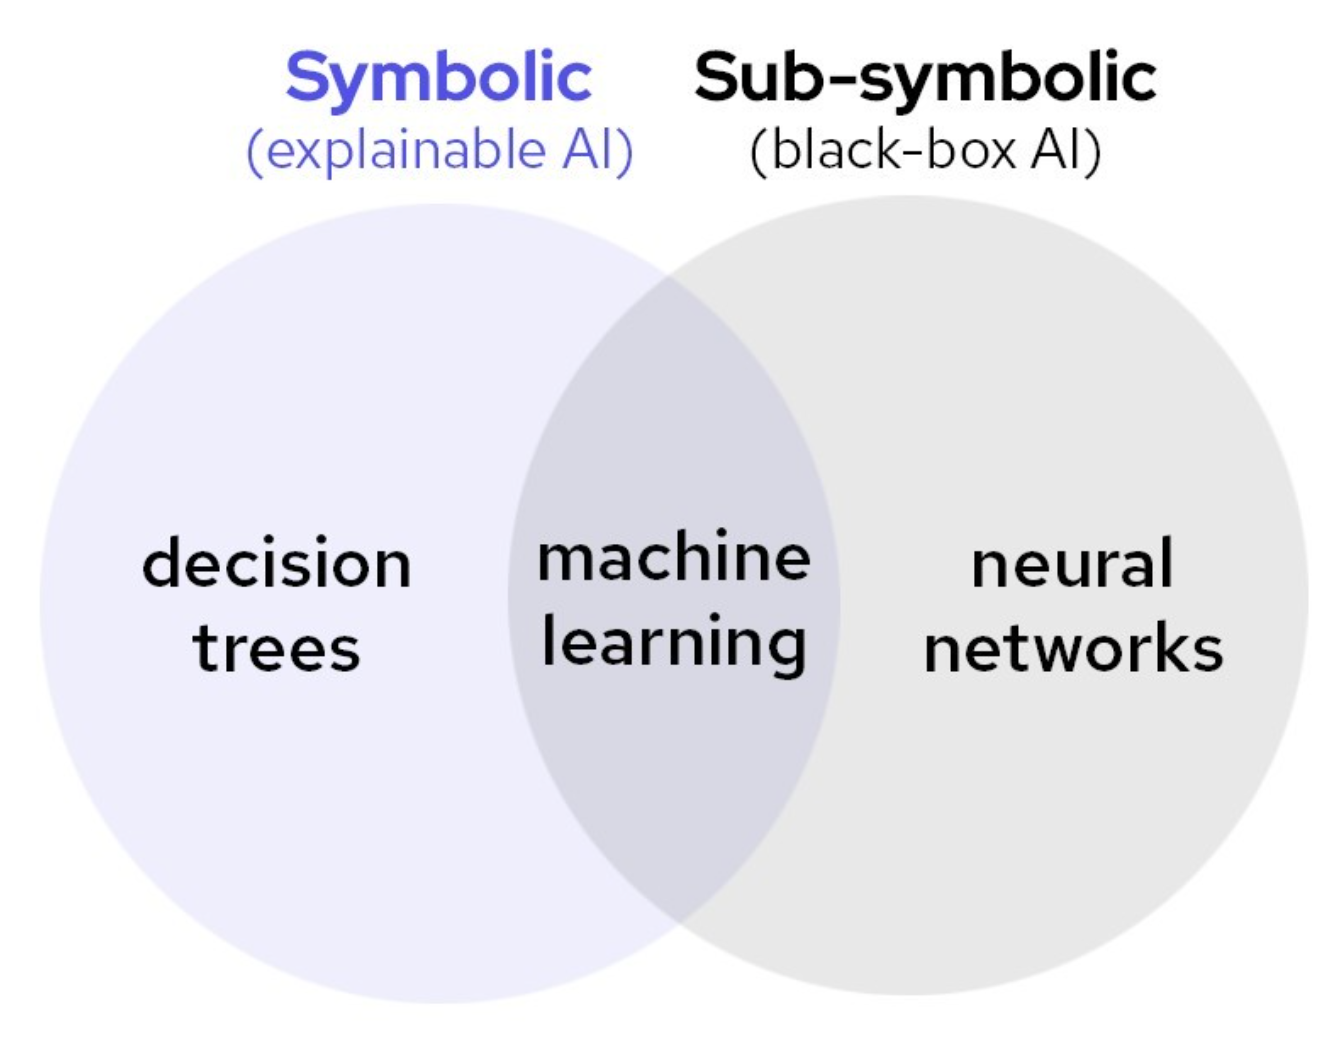
\includegraphics[width=8cm]{../../msml610/lectures_source/figures/L03.symbolic_vs_subsymbolic.png}
  \caption{Symbolic representation encodes knowledge as discrete, labeled
  structure; sub-symbolic representation encodes it as a continuous, learned
  space.}
  \label{fig:symbolic-vs-subsymbolic}
\end{figure}

% From: book_springer/lectures_source/Lesson04.1_Knowledge_Representation.smd:153 '* Neuro-symbolic Approach: Conceptual Spaces'
\textbf{Neuro-symbolic Approach: Conceptual Spaces} --- \emph{Conceptual
spaces} are a neuro-symbolic framework for representing knowledge using
geometric structure rather than discrete symbols alone. Each dimension of
the space corresponds to an interpretable feature, similarity between
objects is modeled as spatial distance rather than as a match or mismatch
between symbols, and a \emph{concept} is not a single point but a region
carved out of this multidimensional space

This geometric framing buys something purely symbolic systems cannot offer
cheaply: a natural way to model similarity and vagueness. A purely symbolic
system represents \texttt{Car} and \texttt{Bicycle} as unrelated discrete
symbols with no structure connecting them, so any claim about how similar
the two are has to be added separately, as an extra fact bolted onto the
representation. A conceptual space, by contrast, places both concepts
somewhere along shared, interpretable dimensions, so the degree of
similarity falls directly out of geometric distance rather than needing to
be stated as an independent axiom

Figure~\ref{fig:conceptual-spaces} works through this with a concrete
example: a conceptual space of transportation methods, organized along two
dimensions, environmental friendliness and technological advancement. Wooden
transportation occupies one region of this space, vehicles occupy a second,
larger region, and advanced vehicles form a nested subset within the
vehicle region, sitting further along the technological-advancement axis.
Nothing about this structure needed to be declared as an explicit rule; the
containment relationships, wooden transportation as a distinct region,
vehicles as a broader category, advanced vehicles as a refinement of it,
emerge from how the regions are positioned and shaped in the space, which is
exactly the kind of graded, geometric structure that a purely symbolic
scheme has no native mechanism for expressing

% rendered_image:begin
% filename: msml610/lectures_source/figures/L03.conceptual_spaces.png
% label: fig:conceptual-spaces
% caption: A conceptual space for transportation methods, with concepts as
%          regions along interpretable dimensions rather than discrete
%          symbols.
% rendered_image:end
\begin{figure}[!t]
  \centering
  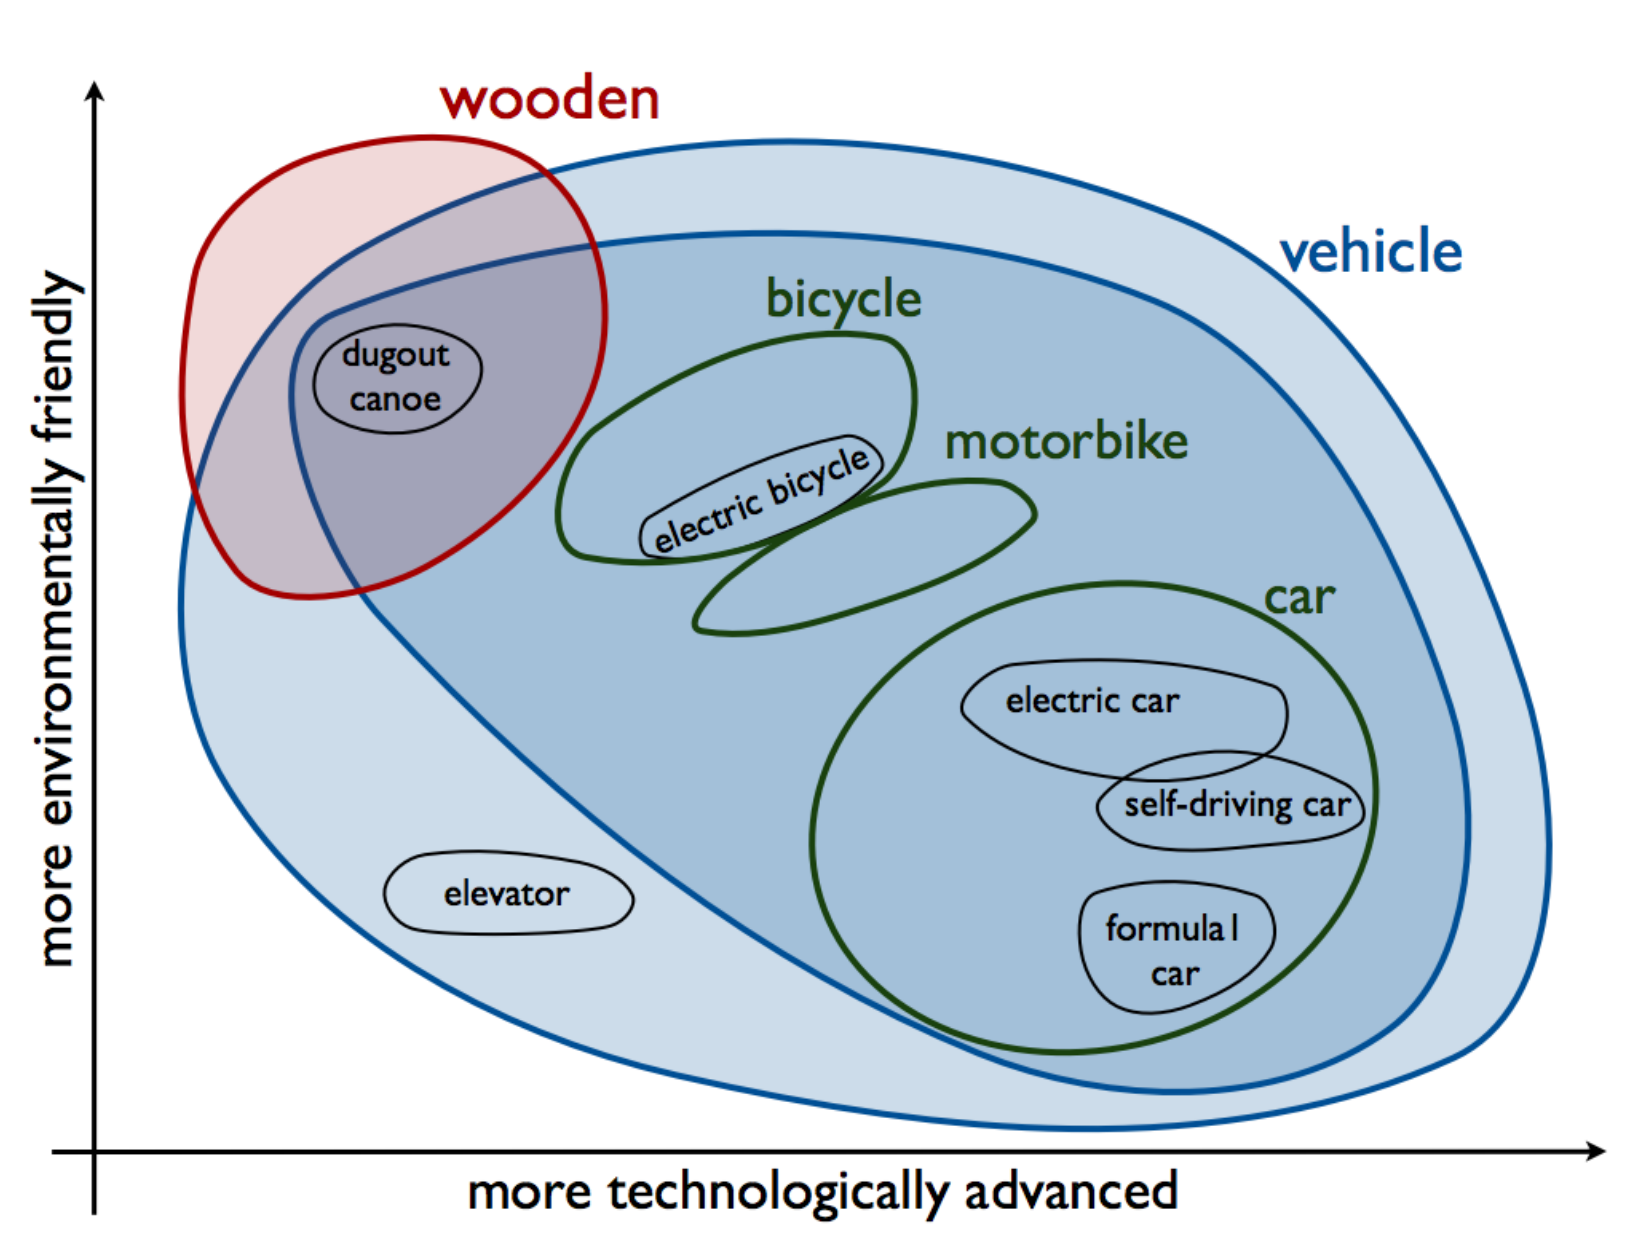
\includegraphics[width=8cm]{../../msml610/lectures_source/figures/L03.conceptual_spaces.png}
  \caption{A conceptual space for transportation methods, with concepts
  represented as regions along interpretable dimensions rather than as
  discrete symbols.}
  \label{fig:conceptual-spaces}
\end{figure}

% From: book_springer/lectures_source/Lesson04.1_Knowledge_Representation.smd:184 '* Procedural vs. Declarative Representation'
\textbf{Procedural vs. Declarative Representation} --- The \emph{procedural
approach} to representing knowledge focuses on \emph{how} a task is done: it
encodes the desired behavior directly into a program, step by step. A robot
programmed with a specific sequence of moves to navigate a maze is a
procedural representation of that navigation task, since the knowledge
\emph{is} the sequence of steps, with no separation between what to
achieve and how to achieve it

The \emph{declarative approach} inverts this: it specifies \emph{what} the
goal is, not \emph{how} to reach it. A declarative representation describes
relationships between actions and goals and leaves the work of finding a
solution to a separate search or inference process. Describing the goal as
``reach the exit of the maze,'' without saying which moves get there, and
letting the robot's planner find a path is a declarative representation of
the same task the procedural example encoded directly

The comparison between the two is a straightforward tradeoff: the
procedural approach offers more direct control over exactly how a task is
carried out but less flexibility, since changing the goal usually means
rewriting the steps; the declarative approach offers more abstraction and is
easier to modify or extend, since changing the goal is a matter of changing
a description rather than a procedure, but it depends on a solver capable
of turning that description into action

Many successful AI systems do not pick one approach over the other; they
use a hybrid, where declarative knowledge is compiled into procedural code
before execution. A planner that takes a declarative goal and generates a
concrete sequence of actions, a plan, is exactly this hybrid pattern in
action: the goal is declared, the mechanism for reaching it is generated
procedurally, and the two representational styles end up working together
rather than in competition

% From: book_springer/lectures_source/Lesson04.1_Knowledge_Representation.smd:207 '* Natural Language as a Representation'
\textbf{Natural Language as a Representation} --- Natural languages such as
English or Italian are a representation scheme humans use constantly, and
they have three properties that make them a poor fit for the kind of formal
reasoning the rest of this chapter builds toward. They are \emph{expressive},
serving primarily as a medium for communication between people rather than
as a representation optimized for machine inference. They are
\emph{ambiguous}: the same word, ``spring,'' can mean a season or a coiled
piece of metal, and nothing in the word itself disambiguates which sense is
meant. And they are \emph{context-dependent}, since the meaning of an
utterance depends on the sentence and situation surrounding it, as with the
single word ``Look!'', whose meaning shifts entirely depending on what is
being pointed at and why

Natural language's influence runs deeper than surface ambiguity, a point
captured by the \emph{Sapir-Whorf hypothesis}: the language a person speaks
shapes how they perceive, think about, and experience the world, and this
shaping happens even through grammatical features that look arbitrary, such
as the gendering of nouns in some languages and not others. If the
hypothesis is right, the representation is not a neutral conduit for
thought; it actively constrains what kinds of thoughts are easy or hard to
have

The clearest illustrations of this constraint come from what languages do
and do not lexicalize. Some languages lack dedicated words for concepts
that other languages express easily, such as certain notions of direction,
while others have many distinct words for a single concept English
collapses into one, as with Arctic languages that distinguish fresh snow
from hard snow with separate terms where English has only ``snow.''
Orwell's invented Newspeak in \emph{1984} pushes this to its logical
extreme as a work of fiction: a language engineered so that certain
concepts, and the thoughts built from them, become literally
unrepresentable to anyone who only has Newspeak's vocabulary to think in

% From: book_springer/lectures_source/Lesson04.1_Knowledge_Representation.smd:231 '* Programming Languages as a Representation'
\textbf{Programming Languages as a Representation} --- A \emph{programming
language} such as \texttt{C++} or \texttt{Python} is itself a formal,
procedural representation scheme: \emph{data structures} represent facts
about the world, and \emph{code} updates those data structures in whatever
way the programmer has decided fits the domain. This makes programming
languages powerful, general-purpose tools, but it also exposes two specific
limitations relative to the KR schemes this chapter is building toward

The first limitation is that programming languages provide no general
mechanism for deriving facts from other facts. Code updates a data
structure according to logic the programmer wrote by hand, based on the
programmer's own domain knowledge, rather than through a domain-independent
inference procedure that could derive new facts from old ones automatically.
The second limitation is expressiveness for partial information: a variable
in a typical programming language holds a single concrete value, or is
undefined, with no built-in way to represent that a fact is only partially
known or to quantify the uncertainty in it. A programming language has no
natural way to encode a statement like ``a white knight is in \texttt{b1}
or in \texttt{f6}'', a genuinely partial piece of information that neither
commits to one square nor leaves the variable completely unset

\emph{Declarative languages} are built to close exactly this gap by keeping
knowledge and inference separate rather than fusing them the way procedural
code does. The \emph{knowledge} component represents the domain-specific
problem, and its meaning is compositional, meaning the meaning of a whole
sentence is built systematically from the meaning of its parts, rather than
handled by ad hoc code. The \emph{inference} component is domain
independent: the same inference procedure, whether it is resolution in
propositional logic or unification in first-order logic, works across any
domain expressed in the language, which is precisely the general mechanism
for deriving facts from facts that a conventional programming language
lacks

% From: book_springer/lectures_source/Lesson04.1_Knowledge_Representation.smd:256 '# Formal Knowledge Representation'
\section{Formal Knowledge Representation}
\label{sec:formal-knowledge-representation}

The previous section established why representation matters and surveyed
the informal spectrum from procedural code to natural language. This
section turns to the formal end of that spectrum: logic-based schemes
designed specifically so that a machine can derive new facts from old ones
through a domain-independent inference procedure. It starts with
propositional logic's syntax and semantics, extends to the quantifiers that
give first-order logic its extra reach, formalizes what it means for one
statement to follow logically from another, and then examines two ways
classical logic's assumptions break down in practice, non-monotonic
reasoning and the closed- versus open-world distinction, before closing
with a framework for learning logical rules directly from examples

% From: book_springer/lectures_source/Lesson04.1_Knowledge_Representation.smd:258 '* Propositional Logic: Syntax and Semantics'
\textbf{Propositional Logic: Syntax and Semantics} --- \begin{definition}
  \emph{Propositional logic} is a formal system for reasoning about
  statements that can be true or false, defined by a \emph{syntax}, which
  fixes the allowable sentences, and a \emph{semantics}, which fixes how
  the truth of a sentence is determined
\end{definition}
The syntax of propositional logic consists of proposition symbols and
logical connectives, so that a sentence such as $P \land Q$ is well formed
because it combines two proposition symbols with a valid connective. The
semantics is the separate question of how the truth of a complex sentence
is evaluated once the truth of its parts is known, typically through truth
tables or deduction rules: if $P$ is true and $Q$ is false, then $P \land
Q$ evaluates to false, regardless of what $P$ and $Q$ actually stand for in
the world

This formal machinery is not merely academic; it underlies several working
technologies. \emph{SAT solvers} are tools for determining whether a
propositional logic formula can be satisfied by some assignment of truth
values, and they are used directly in hardware verification and scheduling
problems, where a design constraint or a scheduling requirement can be
encoded as a formula whose satisfiability answers a concrete engineering
question. \emph{Expert systems} use logic rules to mimic human
decision-making, as in medical diagnosis systems that encode a physician's
if-then knowledge directly as propositional rules. \emph{Rule-based agents}
operate on a set of predefined rules built from this same logical
substrate, as in automated customer service chatbots that route a query
based on which rule's conditions the query satisfies

% From: book_springer/lectures_source/Lesson04.1_Knowledge_Representation.smd:284 '* First-Order Logic: Quantifiers and Inference'
\textbf{First-Order Logic: Quantifiers and Inference} --- Propositional
logic can only talk about named statements one at a time; \emph{quantifiers}
are what let first-order logic express properties of entire collections of
objects at once, instead of enumerating every object by name the way
propositional logic is forced to

The \emph{universal quantifier}, written $\forall x\, P(x)$, makes a
statement about \emph{every} object in the domain: the sentence is true
exactly when $P(x)$ is true for all values of $x$. The \emph{existential
quantifier}, written $\exists x\, P(x)$, makes a weaker claim, that
\emph{some} object, without naming which one, satisfies the property: the
sentence is true as soon as $P(x)$ is true for at least one $x$. These two
quantifiers are what give first-order logic the reach that the earlier
Minesweeper example, restricted to named cells, could never have on its
own

Within a quantified sentence, a variable is either \emph{bound} by a
quantifier or \emph{free}, unbound, and only bound variables have a fixed
logical status independent of context. The sentence $\forall x\,
(Cat(x) \rightarrow Mammal(x))$ binds $x$ under the universal quantifier
and asserts, for every object in the domain, that being a cat implies being
a mammal, a single sentence that stands in for an unboundedly large
conjunction of statements about individual cats, which is exactly the
expressive power that atomic and factored representations, discussed
earlier in this chapter, are structurally unable to provide

% From: book_springer/lectures_source/Lesson04.1_Knowledge_Representation.smd:302 '* Logical Entailment and Inference'
\textbf{Logical Entailment and Inference} --- \begin{definition}
  \emph{Logical entailment} between sentences is the fact that a sentence
  follows logically from another sentence in a knowledge base. ``$\alpha$
  entails $\beta$'', written $\alpha \models \beta$, holds by definition
  exactly when every model in which $\alpha$ is true is also a model in
  which $\beta$ is true, equivalently $M(\alpha) \subseteq M(\beta)$
\end{definition}
Two examples make the definition concrete. In a small ``rain and wet
ground'' world, the sentence $\alpha$: ``$Rain = T, WetGround = T$'' entails
$\beta$: ``$Rain \implies WetGround$''. If it is a fact that it is raining
and the ground is wet, then the conditional rule that rain implies a wet
ground must be true, at least in this particular world; the specific,
concrete fact supports the general conditional rule because every model
consistent with the specific fact is automatically a model in which the
rule holds

A second, purely algebraic example strips away any appeal to intuition
about rain: in a world where $\alpha$ is ``$x = 0$'' and $\beta$ is
``$x \cdot y = 0$'', $\alpha$ entails $\beta$ because in any model where
$x = 0$ holds, $x \cdot y = 0$ holds as well, regardless of what value $y$
happens to take. The entailment goes through purely from the structure of
the two sentences, with no need for the ``sitting table'' world to have any
particular character beyond satisfying $\alpha$

The intuition worth keeping from both examples is that entailment is not a
proof procedure; it is a semantic relationship that ``preserves truth''
across every model consistent with the premise, which makes it a
constraint on what it is consistent to believe. If a knowledge base is
believed, every sentence that base entails must be believed as well, not
because a specific derivation was carried out, but because disbelieving an
entailed sentence while believing the premises that entail it is, by the
definition above, an inconsistent position to hold

% From: book_springer/lectures_source/Lesson04.1_Knowledge_Representation.smd:330 '* Non-Monotonic Logic and Default Reasoning'
\textbf{Non-Monotonic Logic and Default Reasoning} --- \emph{Non-monotonic
logic} is a logic in which adding new information can invalidate
conclusions that were previously derived, a property that separates it
sharply from classical logic. In classical logic, once a conclusion is
proven it remains true no matter what further information arrives; in
non-monotonic logic, conclusions are explicitly allowed to change as new
facts are learned, which is closer to how everyday reasoning actually
behaves

The standard illustration is Tweety the bird. Starting from a knowledge
base containing ``birds typically fly'' and ``Tweety is a bird,'' the
natural conclusion is ``Tweety can fly.'' Adding the new facts ``Tweety is
a penguin'' and ``penguins cannot fly'' does not just add information
alongside the old conclusion, it overturns it, producing the revised
conclusion ``Tweety cannot fly.'' A classical, monotonic logic has no way
to represent this kind of retraction, since a once-derived conclusion is
permanent by construction

This matters because real-world reasoning is built on incomplete or
evolving knowledge almost by default: an agent rarely has the complete
picture up front and has to act on defaults that later facts can override.
Non-monotonic logic gives a system the flexibility to reason under exactly
this condition, drawing a reasonable conclusion from typical-case defaults
while remaining able to revise that conclusion cleanly the moment an
exception, like Tweety turning out to be a penguin, is learned

% From: book_springer/lectures_source/Lesson04.1_Knowledge_Representation.smd:352 '* Open World vs. Closed World Assumptions'
\textbf{Open World vs. Closed World Assumptions} --- \begin{definition}
  The \emph{Closed World Assumption} (CWA) treats any information missing
  from a knowledge base as false by default, an assumption standard in
  relational databases, logic programming, and business rule systems
\end{definition}
Under CWA, if the only recorded fact is ``Alice takes CS101'' and nothing
is said about Bob, the system concludes ``Bob does not take CS101,''
treating the absence of a record as equivalent to a negative fact. This is
exactly the behavior a SQL query expects: a row that is not in the table is
treated as not existing, full stop, which is why CWA is the default
assumption baked into relational databases

\begin{definition}
  The \emph{Open World Assumption} (OWA) treats any information missing
  from a knowledge base as unknown rather than false, an assumption typical
  of the Semantic Web (RDF, OWL) and of incomplete or continuously growing
  data
\end{definition}
Under the identical scenario, ``Alice takes CS101'' known and nothing said
about Bob, OWA concludes only that ``Bob's enrollment is unknown,'' refusing
to treat silence as a negative fact. The choice between CWA and OWA is not
a minor implementation detail: it determines whether a knowledge base that
has not yet recorded a fact is read as denying that fact or merely as not
yet having an opinion on it, which is exactly the kind of decision that has
to be made deliberately when a knowledge base is still growing, as in the
open, decentralized data sources the Semantic Web is built to integrate

% From: book_springer/lectures_source/Lesson04.1_Knowledge_Representation.smd:373 '* Inductive Logic Programming: Learning Rules from Examples'
\textbf{Inductive Logic Programming: Learning Rules from Examples} ---
\begin{definition}
  \emph{Inductive logic programming} (ILP) learns logical rules from
  examples and background knowledge, taking positive and negative examples
  together with background facts and inferring rules that explain them
\end{definition}
Returning to the Tweety scenario one more time illustrates how ILP
operates: given the background knowledge ``birds have wings,'' the positive
example ``Tweety is a bird that can fly,'' and the negative example
``penguin cannot fly,'' ILP infers the rule ``birds can fly unless they are
penguins,'' a rule that explains both the positive and the negative
examples without being told the rule directly

The appeal of this approach is that it produces human-readable rules
rather than an opaque model, integrating learning directly with symbolic
reasoning and letting background knowledge shape what gets learned rather
than forcing every regularity to be rediscovered from raw examples alone.
Set against this, computational complexity grows quickly as the dataset
gets larger, since searching the space of candidate rules that explain a
set of examples is itself an expensive symbolic search; the framework can
still work with noisy, incomplete data to a meaningful degree, but the cost
of the rule search remains the binding constraint on how far ILP scales

% From: book_springer/lectures_source/Lesson04.1_Knowledge_Representation.smd:396 '# Knowledge Representation Frameworks'
\section{Knowledge Representation Frameworks}
\label{sec:knowledge-representation-frameworks}

% From: book_springer/lectures_source/Lesson04.1_Knowledge_Representation.smd:398 '## Description Logics'
\subsection{Description Logics}
\label{subsec:description-logics}

Formal logic supplies the inference machinery; this subsection and the
next turn to the systems built on top of that machinery to represent and
reason about structured domains. Rule-based systems apply logical rules
operationally, grounding connects the symbols those rules manipulate back
to the world they are supposed to describe, and ontologies give the
resulting knowledge a shared vocabulary of classes, individuals, and
relationships that description-logic-style reasoners can check for
consistency and organize into hierarchies

% From: book_springer/lectures_source/Lesson04.1_Knowledge_Representation.smd:402 '* Rule-Based Systems and Knowledge-Based Agents'
\textbf{Rule-Based Systems and Knowledge-Based Agents} --- \begin{definition}
  A \emph{rule-based system} uses ``if-then'' rules to derive conclusions or
  make decisions, mimicking human decision-making by applying logical rules
  to a set of facts
\end{definition}
A rule-based system is built from three components working together: a
\emph{knowledge base}, which stores the facts and rules; an \emph{inference
engine}, which applies rules to known facts to infer new facts or trigger
actions; and \emph{working memory}, which holds the current facts under
consideration at any given point in the reasoning process

The inference engine operates through a repeating cycle:
\begin{enumerate}
  \item \emph{Match}: find every rule whose conditions match the facts
    currently in working memory

  \item \emph{Conflict resolution}: when several rules match at once,
    decide which one to apply

  \item \emph{Act}: apply the chosen rule, which may modify the facts in
    working memory or trigger an external action

  \item \emph{Repeat}: continue the match-resolve-act cycle until no
    further rule applies
\end{enumerate}
A minimal worked example shows the cycle end to end: given the rule ``if a
patient has a fever and a rash, then suggest measles'' and the fact
``patient has a fever and a rash,'' the match step finds the rule
applicable, there is no competing rule to resolve against, and the act step
produces the conclusion ``suggest measles.'' Larger rule-based systems
chain many such cycles together, with the output of one rule feeding the
facts that trigger the next

% From: book_springer/lectures_source/Lesson04.1_Knowledge_Representation.smd:426 '* Grounding: Connecting Symbols to the World'
\textbf{Grounding: Connecting Symbols to the World} --- \begin{definition}
  \emph{Grounding} connects abstract symbols to real-world entities or
  observations, serving as the bridge between a representation stored in a
  knowledge base and the world that representation is meant to describe
\end{definition}
A symbol like \texttt{Apple} in a knowledge base is inert on its own; it
only means something once it is linked to the actual fruit it names, and
that link is exactly what grounding supplies. Without it, a symbolic system
can manipulate \texttt{Apple} according to whatever rules mention the
symbol, perfectly consistently, while having no connection to anything in
the physical world at all

The point of grounding is to make representations meaningful beyond pure
syntax: it is what enables an agent to act meaningfully in the real world
rather than performing purely symbolic manipulation that never touches
anything outside the knowledge base. This is harder than it sounds, because
grounding has to work against noisy, incomplete sensory data and a mapping
from raw inputs to concepts that is itself complex and context dependent, a
camera frame does not arrive pre-labeled with which pixels correspond to
\texttt{Apple}. Grounding is the working assumption behind robotics tasks
such as object recognition and manipulation, behind natural language
understanding, where a word has to be tied to a referent, and behind
autonomous agents and cognitive systems more broadly, wherever a symbol
manipulated internally needs to correspond to something the agent can
sense or affect

% From: book_springer/lectures_source/Lesson04.1_Knowledge_Representation.smd:458 '* Ontologies: Components and Structure'
\textbf{Ontologies: Components and Structure} --- An ontology organizes
domain knowledge through seven kinds of building block, each playing a
distinct structural role
\begin{description}
  \item[Classes / Concepts] represent general concepts in a domain, such as
    \texttt{Person}, \texttt{City}, or \texttt{Car}

  \item[Individuals / Instances] are specific, concrete examples of a
    class, such as \texttt{GP} as an instance of \texttt{Person},
    \texttt{Rome}, or \texttt{Ferrari 458}

  \item[Properties / Relations] describe interactions or associations
    between classes or instances, such as \texttt{isMortal},
    \texttt{locatedIn}, or \texttt{hasAge}

  \item[Attributes / Data values] specify data associated with a specific
    instance, as in the triple (\texttt{GP}, \texttt{hasAge}, a particular
    age value)

  \item[Constraints] are rules that restrict the values a property is
    allowed to take, as in the constraint that (\texttt{Ferrari 458},
    \texttt{mustBe}, \texttt{red})

  \item[Axioms] are logical statements that define rules and constraints
    over the ontology, such as the claim that all humans are mortal,
    $\forall x\, (Person(x) \implies Mortal(x))$

  \item[Hierarchies] organize classes and properties into parent-child
    relationships, as when \texttt{Student} is declared a subclass of
    \texttt{Person}
\end{description}
These seven pieces are not independent add-ons; they compose. An axiom
constrains what a class's instances can be, a hierarchy determines which
axioms and properties an instance inherits from its parent classes, and a
constraint on an attribute is itself expressible as an axiom, which is
exactly the compositional structure that lets an ontology be checked for
consistency and reasoned over automatically, the subject of the next
subsection

% From: book_springer/lectures_source/Lesson04.1_Knowledge_Representation.smd:484 '* Ontologies: A Worked Example (University Domain)'
\textbf{Ontologies: A Worked Example (University Domain)} --- A university
ontology grounds the abstract components from the previous slide in a
single concrete domain. Four classes anchor the ontology: \texttt{Student},
\texttt{Professor}, \texttt{Course}, and \texttt{Department}. Individuals
populate each class: \texttt{Alice} and \texttt{Bob} are instances of
\texttt{Student}; \texttt{GP} and \texttt{DrNo} are instances of
\texttt{Professor}; \texttt{DATA605} and \texttt{MSML610} are instances of
\texttt{Course}; \texttt{ComputerScience} and \texttt{Mathematics} are
instances of \texttt{Department}

Three properties connect these classes into a coherent structure:
\texttt{takesCourse} relates \texttt{Student} to \texttt{Course},
\texttt{teachesCourse} relates \texttt{Professor} to \texttt{Course}, and
\texttt{belongsToDepartment} relates both \texttt{Student} and
\texttt{Professor} to \texttt{Department}. A fourth relation,
\texttt{offersCourse}, runs from \texttt{Department} to \texttt{Course},
closing the loop: a department offers courses, professors who belong to
that department teach some of those courses, and students who belong to
the department, or another one entirely, take them

Two axioms constrain this structure beyond what the class and property
declarations alone specify: every \texttt{Course} must be taught by
exactly one \texttt{Professor}, and every \texttt{Student} must belong to
exactly one \texttt{Department}. Axioms of this kind are what let an
ontology reasoner catch an inconsistency, an instance of \texttt{Course}
with two professors assigned to it, or a \texttt{Student} left without a
\texttt{Department}, violates a stated axiom and can be flagged
automatically, which is exactly the kind of automated consistency checking
that a flat, unstructured collection of facts about students and courses
could never support on its own

\subsection{Reasoning in Ontologies}
\label{subsec:reasoning-in-ontologies}

% From: book_springer/lectures_source/Lesson04.1_Knowledge_Representation.smd:556 '## Reasoning in Ontologies'
Declaring classes, individuals, and axioms is only half of what an ontology
is for; the other half is the set of automated inference tasks that operate
on that structure. This subsection works through the three core reasoning
tasks a description-logic reasoner performs, formalizes description logic
itself as the family of languages these tasks are defined over, and closes
with the standards, RDF, SPARQL, and semantic networks, that let this
machinery scale to knowledge graphs built from many independent sources

% From: book_springer/lectures_source/Lesson04.1_Knowledge_Representation.smd:558 '* Reasoning in Ontologies: Inference Tasks'
\textbf{Reasoning in Ontologies: Inference Tasks} --- Ontology reasoning
rests on three core tasks. \emph{Subsumption} asks ``is class $A$ a
subclass of $B$?'', checking whether one concept is strictly more general
than another; if \texttt{Person} subsumes \texttt{Student}, then every
\texttt{Student} is necessarily a \texttt{Person}, a relationship that is
central to building the taxonomies and hierarchies ontologies depend on

\emph{Satisfiability} asks a different question: ``can an instance of a
concept exist?'', testing whether a concept is logically consistent, free
of contradiction. A concept such as \texttt{FlyingPenguin}, defined to
require flight while also being defined as a penguin, and penguins cannot
fly, is a concept that might turn out not to be satisfiable, since nothing
could simultaneously meet both parts of its definition

\emph{Classification} uses the answers to subsumption checks to organize
concepts automatically into a hierarchy. Given definitions of
\texttt{Animal}, \texttt{Bird}, and \texttt{Penguin}, a classifier does not
need to be told directly that a penguin is a bird and a bird is an animal;
it derives the hierarchy, placing \texttt{Penguin} under \texttt{Bird} and
\texttt{Bird} under \texttt{Animal}, by repeatedly checking which concept
subsumes which, turning subsumption from a pairwise test into a mechanism
for building entire taxonomies automatically

% From: book_springer/lectures_source/Lesson04.1_Knowledge_Representation.smd:581 '* Description Logics and OWL'
\textbf{Description Logics and OWL} --- \begin{definition}
  \emph{Description logic} is a family of languages for representing
  structured knowledge about a domain, positioned deliberately between
  propositional logic and first-order logic: more expressive than the
  former, less expressive, and correspondingly more tractable, than the
  latter
\end{definition}
A description logic is built from three kinds of component: \emph{classes},
abstract groups such as $Person$ or $Animal$; \emph{properties}, binary
relations such as $hasChild$ or $ownsPet$; and \emph{instances}, specific
objects such as $GP$ or GP's dog $Nuvolo$. On top of these components, two
reasoning tasks recur constantly: concept subsumption, ``is class $A$ a
subset of class $B$?'', and instance checking, ``does instance $a$ belong
to class $A$?'', both special cases of the inference tasks introduced above

Syntactically, description logic combines atomic concepts and roles using a
small set of logical constructors, intersection ($\sqcap$), union
($\sqcup$), negation ($\neg$), and the quantifiers $\forall$ and $\exists$,
letting a compound concept be built from simpler ones. The definition
$Father \equiv Man \sqcap \exists hasChild.Person$ reads as ``a father is a
man who has at least one child who is a person,'' a single compound concept
assembled from three primitive pieces using two constructors. Description
logic of this kind is the formal foundation underlying the Web Ontology
Language (OWL), which is used widely to specify ontologies that other
systems can reason over automatically

% From: book_springer/lectures_source/Lesson04.1_Knowledge_Representation.smd:605 '* RDF and SPARQL: Representation Standards'
\textbf{RDF and SPARQL: Representation Standards} --- The Resource
Description Framework (RDF) represents knowledge as statements that form
directed graphs of nodes and edges, where each node or edge is identified
by a globally unique URI, or carries a literal value, ensuring that a
symbol such as \texttt{http://example.org/Nuvolo} refers to exactly one
thing no matter which system or organization is making the statement. This
global uniqueness is precisely what lets RDF graphs published by different
sources be merged into a single, larger graph without symbol names
colliding by accident, the property that makes RDF a viable substrate for
knowledge built collaboratively rather than by one closed system

SPARQL is the query language built for exactly this kind of graph,
providing the same role for RDF that SQL provides for relational tables:
a way to retrieve and combine facts out of a graph that may be far larger
than any one query needs to touch. Together, RDF and SPARQL underlie
building knowledge graphs from many independent, mergeable sources,
supporting semantic search over that graph, and supporting the
ontology-based reasoning described earlier in this subsection, since an
ontology's classes and axioms can themselves be stored and queried as RDF
statements

% From: book_springer/lectures_source/Lesson04.1_Knowledge_Representation.smd:618 '* Semantic Networks and Knowledge Graphs'
\textbf{Semantic Networks and Knowledge Graphs} --- \begin{definition}
  \emph{Semantic networks} represent knowledge as graphs of concepts and
  the relations between them
\end{definition}
A semantic network is built from two kinds of component: \emph{nodes},
which represent concepts, and \emph{edges}, which represent relations
between those concepts, such as ``is-a'' or ``part-of.'' The edge
\texttt{Dog is Animal}, for instance, does not just record a fact; it
licenses \texttt{Dog} to inherit whatever traits are attached to
\texttt{Animal}, which is what makes a semantic network more than a static
diagram, it is a structure inference can walk across

WordNet and ConceptNet are two well-known instances of this idea at scale,
each a large semantic network of lexical or commonsense concepts linked by
typed relations. Their appeal is largely practical: a semantic network is
easy to visualize and traverse, its graph structure supports reasoning
directly, whether by following ``is-a'' edges to inherit properties or by
searching for paths that connect two concepts, and this combination of
visual clarity and reasoning support is why semantic networks appear both
in early AI systems and in today's large-scale knowledge graph
applications

% From: book_springer/lectures_source/Lesson04.1_Knowledge_Representation.smd:637 '# Graphical Models for Uncertainty'
\section{Graphical Models for Uncertainty}
\label{sec:graphical-models-uncertainty}

Logic, in every form covered so far in this chapter, reasons about
statements that are true or false, with no native slot for a statement
that is merely likely. Real agents rarely have that luxury: the world they
act in is only partially observable, does not respond deterministically to
their actions, and sometimes contains other agents actively working against
them. This section introduces the representational fix, Bayesian
networks, which keep the graph-based structure that ontologies and
semantic networks already established but replace hard logical rules with
probability distributions that can represent degrees of belief rather than
only certainties

% From: book_springer/lectures_source/Lesson04.1_Knowledge_Representation.smd:639 '* Why Logic Fails Under Uncertainty'
\textbf{Why Logic Fails Under Uncertainty} --- Logic-based AI systems, built
on propositional logic, typically represent actions using rules of the
form ``if preconditions $P$ hold, then action $A$ causes effect $E$.'' The
rule ``if I turn the car key, the engine starts'' is a rule of exactly this
shape, and it is usually a perfectly good description of what happens

The trouble is what the rule leaves out: the battery might be dead, there
might be no fuel, the starter might be broken, and any of these
possibilities breaks the clean if-then relationship the rule asserts,
without the rule itself having any way to express how likely each failure
mode is or what to conclude when the key turns and the engine does not
start. This is not a flaw specific to car engines; it is structural.
Real-world agents face uncertainty for three distinct reasons: \emph{partial
observability}, where the agent cannot see the full state of the world it
is acting in; \emph{non-determinism}, where actions do not always produce
deterministic or fully predictable outcomes even when the relevant state is
known; and \emph{adversarial conditions}, where other agents may actively
interfere with the expected outcome. A purely logical rule, built to say
that a precondition guarantees an effect, has no native way to represent
any of these three sources of uncertainty, which is exactly the gap
graphical models are built to close

% From: book_springer/lectures_source/Lesson04.1_Knowledge_Representation.smd:659 '* Bayesian Networks: Definition and Structure'
\textbf{Bayesian Networks: Definition and Structure} --- Bayesian networks
appear in the literature under several names, Bayes nets, belief networks,
probabilistic networks, and, as the broader class that networks with only
causal edges belong to, graphical models; when the arrows are given a
specific causal meaning, the same structure is called a causal network,
the topic of the next section
\begin{definition}
  A \emph{Bayesian network} is a Directed Acyclic Graph (DAG) whose nodes
  $X_i$ correspond to random variables, discrete or continuous, and whose
  edges $X \to Y$ connect nodes to represent dependencies among variables,
  such as $X$ being a parent of $Y$, $Y$ being a child of $X$, or the two
  being ancestors or spouses of one another within the graph
\end{definition}
Every node in the network is associated with a conditional probability
table (CPT, also called a CPD), quantifying how its parents affect it:
\begin{equation}
  \label{eq:bayesian-network-cpt}
  \Pr(X_i \mid Parents(X_i))\;.
\end{equation}
A node with no parents at all is simply given a prior probability instead
of a conditional one, since Eq.~\eqref{eq:bayesian-network-cpt} degenerates
to an unconditional distribution when the parent set is empty. This local
structure, one small conditional table per node, is what makes Bayesian
networks tractable despite representing a full joint distribution over
every variable in the graph: the DAG's edges specify exactly which
variables each node's probability depends on, so the full joint
distribution can be reconstructed by multiplying together these local,
manageable pieces rather than having to be specified directly

% From: book_springer/lectures_source/Lesson04.1_Knowledge_Representation.smd:674 '# Causal Graphical Models'
\section{Causal Graphical Models}
\label{sec:causal-graphical-models-kr}

A Bayesian network's edges encode statistical dependence, not necessarily
cause and effect, a distinction this section makes precise. Restricting a
Bayesian network's edges to represent only genuine causal relationships
produces a causal network, a structure this section defines formally
before working through what that added causal commitment buys, in terms of
reasoning about interventions, and how it can be made fully quantitative
through structural causal models

% From: book_springer/lectures_source/Lesson04.1_Knowledge_Representation.smd:676 '* Causal Networks (Causal DAGs): Definition and Structure'
\textbf{Causal Networks (Causal DAGs): Definition and Structure} --- A
causal DAG carries two structural properties in its name. It is
\emph{directed}: arrows point from cause to effect, not merely between
correlated variables. It is \emph{acyclic}: no feedback loops are allowed,
because causal relationships assume a temporal order in which cause
precedes effect, and a cycle would require a variable to be both the cause
and the effect of itself, which is not a coherent causal claim

Committing to this stricter, causal reading of the graph's edges buys real
benefits. A causal DAG makes causal links explicit rather than leaving them
implicit in a correlational structure, which supports explainable AI models
whose outputs can be traced back to specific causal mechanisms. It brings
stability to conditional probability estimation, since a genuinely causal
relationship tends to hold up under distribution shift in a way a merely
correlational one does not. And, most importantly for the sections that
follow, it supports reasoning about interventions and counterfactuals,
questions a purely statistical Bayesian network is not equipped to answer.
These benefits come with real limitations: building a causal DAG requires
domain knowledge to get the edge directions right in the first place, and
the resulting graph is only as good as its assumption that all relevant
variables are included, with no hidden confounders lurking outside the
graph and distorting the causal picture it presents

% From: book_springer/lectures_source/Lesson04.1_Knowledge_Representation.smd:695 '* The Ladder of Causation: Association, Intervention, Counterfactual'
\textbf{The Ladder of Causation: Association, Intervention, Counterfactual}
--- A causal DAG is easiest to read through a concrete example: a severe
weather alert reaching the public. The causal chain runs through five
variables: $T$, a tornado forming; $W$, the National Weather Service
issuing a tornado warning in response; $A$ and $B$, radio and television
broadcasting the emergency; and $R$, residents actually being warned. The
DAG connects them as $T \to W$, $W \to A$, $W \to B$, and both $A \to R$ and
$B \to R$, a chain from tornado formation through the warning system's two
broadcast channels to the residents it is meant to reach

The example is built on three assumptions that make the causal chain
clean: the broadcast channels transmit only on an official warning order,
never independently; the delivery systems never fail once triggered; and
residents are warned as soon as either broadcast channel activates, so the
two channels are redundant rather than both required. This structure
illustrates the three rungs the ladder of causation distinguishes. Read
purely associationally, the graph says which variables move together.
Read as an intervention, it supports asking what happens to $R$ if $W$ is
forced to occur regardless of $T$, pulling the warning lever directly
rather than merely observing it. Read counterfactually, it supports asking
whether a specific set of residents would have been warned had the warning
never been issued, a question about a specific case that did not occur,
not about the graph's typical behavior in general

% From: book_springer/lectures_source/Lesson04.1_Knowledge_Representation.smd:746 '* Structural Causal Models (SCM): Definition'
\textbf{Structural Causal Models (SCM): Definition} --- \begin{definition}
  A \emph{Structural Causal Model} (SCM) translates a causal DAG into
  mathematical equations that define how the variables in the graph
  interact
\end{definition}
An SCM represents each variable $X_1, X_2, \ldots, X_n$ in the system as a
function of its direct causes:
\begin{equation}
  \label{eq:scm-structural-equation}
  X_i = f_i\bigl(Parents(X_i), \varepsilon_i\bigr)\;,
\end{equation}
where $Parents(X_i)$ are $X_i$'s direct causes in the DAG and $\varepsilon_i$
is an exogenous, unobserved noise term standing in for every influence on
$X_i$ that the model does not represent explicitly. Equation
\eqref{eq:scm-structural-equation} is what turns a causal DAG's qualitative
arrows into something that can actually be simulated or intervened on: the
DAG says which variables are causes of $X_i$, and the SCM says precisely
how those causes combine to produce $X_i$'s value

An SCM inherits every property a causal network already has, explaining
causal relationships between variables and providing a foundation for
causal reasoning and simulation, and adds the ability to quantify the
effect precisely rather than only asserting that a causal link exists.
This combination of a DAG's structure with explicit functional equations
is not a recent methodological fashion, structural equation models of this
kind have been used in econometrics and genetics for a long time, well
before causality was formalized as a distinct branch of statistics and
computer science, which is worth remembering when SCMs are introduced as
though they were a purely computational innovation

% From: book_springer/lectures_source/Lesson04.1_Knowledge_Representation.smd:771 '# Integrating Logic and Causality'
\section{Integrating Logic and Causality}
\label{sec:integrating-logic-causality}

This chapter opened with symbolic logic and moved, section by section,
toward the probabilistic and causal graphical models needed to represent
uncertainty and intervention. This closing section brings the two threads
back together: Markov logic networks attach probabilistic weights directly
to first-order logic formulas, and revisiting Bayesian networks one more
time, now explicitly against causal networks, shows precisely what a
causal reading of a graph's edges adds on top of the purely statistical
one

% From: book_springer/lectures_source/Lesson04.1_Knowledge_Representation.smd:773 '* Markov Logic Networks: Combining Logic and Probability'
\textbf{Markov Logic Networks: Combining Logic and Probability} --- A
\emph{Markov Logic Network} (MLN) combines first-order logic, which
expresses knowledge through rules and quantifiers, with Markov Random
Fields, which model uncertainty through probabilities, into a single
representation. An MLN is a set of pairs $(F_i, w_i)$, where $F_i$ is a
first-order logic formula, such as $Friends(x,y) \implies Similar(x,y)$,
and $w_i$ is a weight measuring the strength of belief in $F_i$: a higher
$w_i$ makes the formula more influential in shaping the resulting
probability distribution

Semantically, an MLN defines a probability distribution over
\emph{possible worlds}, where a world is a complete assignment of truth
values to every ground atom in the domain. A world that satisfies many
high-weight formulas becomes more probable under this distribution than
one that violates them, which is what lets an MLN prefer worlds that
respect its rules without treating any rule as an absolute, inviolable
constraint. Formally, the joint distribution takes the form
\begin{equation}
  \label{eq:mln-joint-distribution}
  \Pr(X = x) = \frac{1}{Z} \exp\left(\sum_i w_i\, n_i(x)\right)\;,
\end{equation}
where $n_i(x)$ counts the number of \emph{true groundings} of formula
$F_i$ in world $x$. If $F_i$ is $Friends(x,y) \implies Similar(x,y)$ and
this implication holds for 7 out of 10 possible $(x,y)$ pairs in a
particular world, then $n_i(x) = 7$ for that world, and
Eq.~\eqref{eq:mln-joint-distribution} rewards worlds with a higher count
proportionally to the formula's weight $w_i$

Two special cases situate MLNs relative to classical logic. If every
weight $w_i \to \infty$, only worlds in which all formulas are fully
satisfied retain any nonzero probability, and the MLN collapses exactly
onto classical logic, where a single violated rule is enough to rule a
world out entirely. If every weight stays finite, the MLN allows some
formulas to be violated while assigning worlds that violate more, or
higher-weight, formulas a correspondingly lower probability, which is the
soft, graded behavior that distinguishes an MLN from the hard constraints
of classical first-order logic it is built from

% From: book_springer/lectures_source/Lesson04.1_Knowledge_Representation.smd:816 '* From Correlation to Causal Reasoning: What Graphs Add'
\textbf{From Correlation to Causal Reasoning: What Graphs Add} --- A
Bayesian network represents a joint distribution function, and the
direction its arrows point represents conditional dependence, not
causality: an edge $A \to B$ simply requires estimating $\Pr(A \mid B)$ as
part of the network's factorization, with no claim built in about which
variable causes which. This has a direct consequence: many different
Bayesian networks, with the same nodes but different edges, can explain
the identical phenomenon equally well

Two variables, $Fire$ and $Smoke$, which are statistically dependent, make
this concrete. A network with $Fire \to Smoke$ requires $\Pr(Fire)$ and
$\Pr(Smoke \mid Fire)$ to reconstruct the joint distribution $\Pr(Fire,
Smoke)$. A network with the edge reversed, $Smoke \to Fire$, requires
instead $\Pr(Smoke)$ and $\Pr(Fire \mid Smoke)$. Both networks reproduce
the same joint distribution over $Fire$ and $Smoke$, are statistically
equivalent, and convey the same information about which variables are
dependent, yet they differ in how difficult each conditional distribution
actually is to estimate from data, one direction may be far easier to fit
than the other even though both are formally valid factorizations

What breaks the tie between the two directions is not statistics but an
asymmetry in nature: extinguishing the fire stops the smoke, but clearing
the smoke away does not affect the fire, an asymmetry no amount of
correlational data alone can reveal, since both directions fit the same
joint distribution equally well. A \emph{causal network} is a Bayesian
network restricted to edges that respect this kind of real-world asymmetry,
which requires judgment grounded in how the system actually works, not
just in which statistical factorization happens to be convenient. Making
this judgment means shifting the question from ``are $Smoke$ and $Fire$
correlated?'', a question the data alone answers, to ``what causes what,
$Smoke$ or $Fire$?'', a question that needs an external, causal
commitment

This causal commitment can be stated with the same directness as an
assignment statement in a program: nature assigns $Smoke$ as a function of
$Fire$, $Smoke := f(Fire)$, and not the other way around, $Fire := f(Smoke)$
is simply the wrong assignment for how fire and smoke actually relate.
\emph{Structural equations} formalize exactly this ``assignment
mechanism'' inside a causal graph:
\begin{equation}
  \label{eq:causal-assignment-mechanism}
  X_i := f(X_j) \iff X_j \to X_i\;,
\end{equation}
tying every causal edge in the graph to a directional assignment rather
than to a merely symmetric statistical dependency, which is precisely the
distinction, first raised at the top of this section, between a Bayesian
network's arrows and a causal network's arrows: the same graphical
notation, carrying a strictly stronger claim

%\include{chapter}
%\include{appendix}

\backmatter%%%%%%%%%%%%%%%%%%%%%%%%%%%%%%%%%%%%%%%%%%%%%%%%%%%%%%%
%\include{glossary}
%\include{solutions}
%\printindex

%%%%%%%%%%%%%%%%%%%%%%%%%%%%%%%%%%%%%%%%%%%%%%%%%%%%%%%%%%%%%%%%%%%%%%

\end{document}
